\documentclass[12pt, letterpaper]{report}

% =========================================================
% FORMATO PUCV
% =========================================================

\usepackage{pucv_inf_2024}
\usepackage{tikz}

% Idioma: partición silábica en español.
% Solo se activa si la distribución de LaTeX tiene instalado el idioma
% (paquete 'texlive-langspanish' o equivalente). Sin él, el documento
% compila igual, pero la separación silábica usa las reglas del inglés.
\IfFileExists{spanish.ldf}{%
    \usepackage[spanish, es-tabla, es-noshorthands]{babel}%
}{}

% =========================================================
% PAQUETES ADICIONALES
% =========================================================

\usepackage{graphicx}
\usepackage{float}
\usepackage{booktabs}
\usepackage{tabularx}
\usepackage{array}
\usepackage{longtable}
\usepackage{multirow}
\usepackage{colortbl}
\usepackage{pdflscape}
\usepackage{adjustbox}
\usepackage{ulem}
\normalem
\usepackage[most]{tcolorbox}
\usepackage[hidelinks]{hyperref}

\graphicspath{{Figuras/}}

% =========================================================
% ESTILOS PROPIOS DEL INFORME (incluye estilos TikZ)
% =========================================================

% =========================================================
% ESTILOS Y COMANDOS PROPIOS DEL INFORME
% Complementa a pucv_inf_2024.sty sin modificarlo.
% =========================================================

% ---------------------------------------------------------
% Rótulos en español
% Se reaplican después de babel para conservar los títulos de
% índices definidos por pucv_inf_2024.sty.
% ---------------------------------------------------------

\AtBeginDocument{%
    \renewcommand{\figurename}{Figura}%
    \renewcommand{\tablename}{Tabla}%
    \renewcommand{\nomname}{\uppercase{Lista de Símbolos}}%
    \renewcommand{\contentsname}{\uppercase{Índice General}}%
    \renewcommand{\listfigurename}{\uppercase{Lista de Figuras}}%
    \renewcommand{\listtablename}{\uppercase{Lista de Tablas}}%
    \renewcommand{\chaptername}{Capítulo}%
    \renewcommand{\appendixname}{Anexo}%
    \renewcommand{\partname}{Parte}%
}

% ---------------------------------------------------------
% Bibliografía en español
% Fuerza los rótulos APA en español («Recuperado el ... de»,
% «2.ª ed.», «y» en lugar de «and») sin depender de babel.
% ---------------------------------------------------------

\ExecuteBibliographyOptions{language = spanish}
\DeclareLanguageMapping{spanish}{spanish-apa}

% ---------------------------------------------------------
% Colores auxiliares
% ---------------------------------------------------------

\definecolor{notacolor}{HTML}{4472c4}   % azul institucional (igual a titlecolor)
\definecolor{notafondo}{HTML}{EEF2FA}
\definecolor{pendientecolor}{HTML}{B85C00}
\definecolor{pendientefondo}{HTML}{FDF3E7}
\definecolor{filacabecera}{HTML}{DCE6F5}

% ---------------------------------------------------------
% Cajas de nota y de tareas pendientes
% (equivalen a las citas en bloque y a los bloques
%  "POR COMPLETAR" del documento original en Markdown)
% ---------------------------------------------------------

\newtcolorbox{nota}[1][]{%
    enhanced,
    breakable,
    colback = notafondo,
    colframe = notacolor,
    boxrule = 0pt,
    leftrule = 3pt,
    arc = 0pt,
    outer arc = 0pt,
    left = 8pt, right = 8pt, top = 6pt, bottom = 6pt,
    fontupper = \small,
    parbox = false,
    #1
}

\newtcolorbox{pendiente}[1][Por completar]{%
    enhanced,
    breakable,
    colback = pendientefondo,
    colframe = pendientecolor,
    boxrule = 0.6pt,
    arc = 2pt,
    left = 8pt, right = 8pt, top = 6pt, bottom = 6pt,
    fontupper = \small,
    parbox = false,
    title = {\footnotesize\bfseries\MakeUppercase{#1}},
    coltitle = white,
    colbacktitle = pendientecolor
}

% Marca breve, para usar dentro de una línea de texto
\newcommand{\porcompletarinline}[1]{%
    \textcolor{pendientecolor}{\textbf{[por completar: #1]}}%
}

% ---------------------------------------------------------
% Estilo común de las tablas largas
% ---------------------------------------------------------

\newcommand{\estilotabla}{%
    \footnotesize
    \setlength{\parskip}{0pt}%
    \setlength{\parindent}{0pt}%
    \setlength{\tabcolsep}{4pt}%
    \renewcommand{\arraystretch}{1.25}%
}

\newcommand{\estilotablachica}{%
    \estilotabla
    \scriptsize
}

% Separación antes y después de las longtable
\setlength{\LTpre}{8pt}
\setlength{\LTpost}{8pt}

% Columnas de párrafo centradas verticalmente arriba
\newcolumntype{L}[1]{>{\raggedright\arraybackslash}p{#1}}
\newcolumntype{C}[1]{>{\centering\arraybackslash}p{#1}}

% ---------------------------------------------------------
% Identificadores de código, clases y estados
% ---------------------------------------------------------

\newcommand{\clase}[1]{\texttt{#1}}
\newcommand{\estado}[1]{\texttt{#1}}
\newcommand{\este}[1]{\textit{#1}}

% Estereotipos UML
\newcommand{\ster}[1]{\texttt{\guillemotleft #1\guillemotright}}

% ---------------------------------------------------------
% Figuras de diagramas: comando abreviado
% #1 ancho relativo · #2 archivo · #3 título breve (Lista de Figuras)
% #4 leyenda completa · #5 etiqueta
% ---------------------------------------------------------

\newcommand{\figuradiagrama}[5]{%
    \begin{figure}[H]
        \centering
        \IfFileExists{Figuras/diagramas/#2}{%
            \includegraphics[width=#1\textwidth]{#2}%
        }{%
            \fbox{\parbox[c][7cm][c]{0.85\textwidth}{\centering
                \textbf{[Diagrama pendiente]}\\[4pt]
                \texttt{Figuras/diagramas/#2}}}%
        }
        \caption[#3]{#4}
        \label{#5}
    \end{figure}%
}

% ---------------------------------------------------------
% Tablas de casos de uso narrativos (formato de los ejemplos)
% ---------------------------------------------------------

\newcommand{\campocu}[2]{\hline \textbf{#1} & #2 \\}
\newcommand{\encabezadocu}[1]{\hline \rowcolor{filacabecera} \multicolumn{2}{|c|}{\textbf{#1}} \\}
\newcommand{\subencabezadocu}[2]{\hline \rowcolor{filacabecera} \textbf{#1} & \textbf{#2} \\}

% ---------------------------------------------------------
% Ajustes de listas y espaciado dentro de entornos
% ---------------------------------------------------------

\setlist[itemize]{leftmargin=1.2cm, itemsep=2pt, topsep=4pt}
\setlist[enumerate]{leftmargin=1.2cm, itemsep=2pt, topsep=4pt}

% Evita que hyperref rompa las referencias de longtable
\hypersetup{
    bookmarksnumbered = true,
    pdftitle = {Informe 3 - Análisis y diseño estructurado del sistema BeeTracer},
    pdfsubject = {ICI-3242 Modelamiento de Software - PUCV}
}

% Nombre de botón o menú entre comillas angulares
\newcommand{\bt}[1]{\guillemotleft{}#1\guillemotright{}}

% Numeración corrida de figuras y tablas (Figura 1, 2, 3... como en los ejemplos)
\usepackage{chngcntr}
\counterwithout{figure}{chapter}
\counterwithout{table}{chapter}

% ---------------------------------------------------------
% Tolerancia de justificación: evita desbordes de línea con
% nombres de clases largos en monoespaciado.
% ---------------------------------------------------------

\setlength{\emergencystretch}{3em}

% ---------------------------------------------------------
% Páginas de "Parte" (Parte 1: Análisis · Parte 2: Diseño)
% ---------------------------------------------------------

\renewcommand{\thepart}{\arabic{part}}
\titleformat{\part}[display]
    {\centering\normalfont\bfseries\Huge\color{titlecolor}}
    {\MakeUppercase{\partname}~\thepart}{1em}{\MakeUppercase}

% ---------------------------------------------------------
% Estilos TikZ para los diagramas del análisis y diseño
% estructurado (notación de Yourdon/DeMarco, Chen y
% diagramas de estructura de Yourdon y Constantine)
% ---------------------------------------------------------

\usetikzlibrary{arrows.meta, positioning, calc, fit, backgrounds,
    shapes.geometric, shapes.multipart, decorations.markings}

\definecolor{dfdproceso}{HTML}{EAF1FB}
\definecolor{dfdterminador}{HTML}{E6E6E6}
\definecolor{dfdalmacen}{HTML}{FFF8E6}
\definecolor{dfdborde}{HTML}{2F4F7F}

\tikzset{
    % --- Diagramas de flujo de datos ---
    proceso/.style = {circle, draw = dfdborde, line width = 0.7pt,
        fill = dfdproceso, align = center, font = \scriptsize,
        minimum size = #1, inner sep = 1pt},
    proceso/.default = 2.3cm,
    terminador/.style = {rectangle, draw = black, line width = 0.7pt,
        fill = dfdterminador, align = center, font = \scriptsize\bfseries,
        minimum width = 2.5cm, minimum height = 0.95cm, inner sep = 3pt},
    almacen/.style = {rectangle, fill = dfdalmacen, align = center,
        font = \scriptsize, minimum width = #1, minimum height = 0.6cm,
        inner sep = 2pt, outer sep = 0pt,
        append after command = {
            (\tikzlastnode.north west) edge[draw, -, line width = 0.8pt]
            (\tikzlastnode.north east)
            (\tikzlastnode.south west) edge[draw, -, line width = 0.8pt]
            (\tikzlastnode.south east)}},
    almacen/.default = 2.6cm,
    flujo/.style = {-{Stealth[length = 2mm]}, line width = 0.5pt},
    etq/.style = {font = \tiny, fill = white, inner sep = 1pt,
        align = center, text = black},
    % --- Diagrama entidad-relación (Chen) ---
    entidad/.style = {rectangle split, rectangle split parts = 2,
        draw = black, line width = 0.7pt,
        font = \scriptsize, inner sep = 2.5pt, minimum width = 3.0cm, align = left,
        rectangle split part align = {center, left},
        rectangle split part fill = {dfdborde!22, white}},
    relacion/.style = {diamond, aspect = 2.4, draw = black,
        line width = 0.6pt, fill = dfdalmacen, font = \scriptsize,
        align = center, inner sep = 0.5pt},
    card/.style = {font = \scriptsize\bfseries, inner sep = 1pt, fill = white},
    % --- Modelo relacional ---
    tabla/.style = {rectangle split, rectangle split parts = 2,
        draw = black, line width = 0.6pt, font = \tiny, align = left,
        inner sep = 2pt, rectangle split part fill = {dfdborde!30, white},
        rectangle split part align = {center, left}},
    fk/.style = {-{Stealth[length = 1.6mm]}, line width = 0.45pt,
        draw = dfdborde},
    % --- Diagramas de estructura ---
    modulo/.style = {rectangle, draw = black, line width = 0.7pt,
        fill = dfdproceso, align = center, font = \scriptsize,
        text width = #1, minimum height = 0.9cm, inner sep = 2pt,
        execute at begin node = {\hyphenpenalty = 10000 \exhyphenpenalty = 10000}},
    modulo/.default = 2.1cm,
    predefinido/.style = {modulo = #1,
        append after command = {
            ($(\tikzlastnode.north west) + (0.12, 0)$) edge[draw, -, line width = 0.5pt]
            ($(\tikzlastnode.south west) + (0.12, 0)$)
            ($(\tikzlastnode.north east) + (-0.12, 0)$) edge[draw, -, line width = 0.5pt]
            ($(\tikzlastnode.south east) + (-0.12, 0)$)}},
    predefinido/.default = 2.1cm,
    llamada/.style = {-{Stealth[length = 1.8mm]}, line width = 0.5pt},
    dato/.style = {{Circle[open, length = 1.6mm]}-{Stealth[length = 1.6mm]},
        line width = 0.4pt},
    control/.style = {{Circle[length = 1.6mm]}-{Stealth[length = 1.6mm]},
        line width = 0.4pt},
    acop/.style = {font = \tiny, inner sep = 0.8pt, align = center},
}

% Rótulo de proceso: número en negrita y nombre debajo
\newcommand{\proc}[2]{\textbf{#1}\\[-1pt]#2}

% Inclusión de un diagrama TikZ ajustado al ancho disponible
% #1 archivo en Figuras/tikz · #2 título breve · #3 leyenda · #4 etiqueta
\newcommand{\diagramatikz}[4]{%
    \begin{figure}[H]
        \centering
        \begin{adjustbox}{max width=\textwidth, max totalheight=0.80\textheight}
            \input{Figuras/tikz/#1}
        \end{adjustbox}
        \caption[#2]{#3}
        \label{#4}
    \end{figure}%
}

% Par de flujos opuestos entre un terminador (o almacén) y un proceso.
% #1 punto origen (externo) · #2 punto destino (proceso)
% #3 rótulo del flujo #1->#2 · #4 rótulo del flujo #2->#1
% #5 posición del rótulo #3 · #6 posición del rótulo #4 (0 a 1)
\newcommand{\parflujo}[6]{%
    \draw[flujo] ($(#1)!0.17cm!90:(#2)$) --
        node[etq, auto, pos = #5] {#3} ($(#2)!0.17cm!-90:(#1)$);
    \draw[flujo] ($(#2)!0.17cm!90:(#1)$) --
        node[etq, auto, pos = #6] {#4} ($(#1)!0.17cm!-90:(#2)$);
}

% Flujo de lectura y escritura sobre un almacén (doble punta)
\tikzset{flujorw/.style = {{Stealth[length = 2mm]}-{Stealth[length = 2mm]},
    line width = 0.5pt}}

% Diagrama TikZ en página apaisada
% #1 archivo · #2 título breve · #3 leyenda · #4 etiqueta
\newcommand{\diagramaapaisado}[4]{%
    \begin{landscape}
    \begin{figure}[p]
        \centering
        \begin{adjustbox}{max width=\linewidth, max totalheight=0.86\textheight}
            \input{Figuras/tikz/#1}
        \end{adjustbox}
        \caption[#2]{#3}
        \label{#4}
    \end{figure}
    \end{landscape}%
}

% Relación del DER entre dos entidades con su rombo y cardinalidades
% #1 entidad A · #2 entidad B · #3 nombre del rombo · #4 rótulo
% #5 cardinalidad junto a A · #6 cardinalidad junto a B · #7 posición del rombo
\newcommand{\relER}[7]{%
    \node[relacion] (#3) at ($(#1)!#7!(#2)$) {#4};
    \draw[line width = 0.5pt] (#1) -- node[card, pos = 0.4] {#5} (#3);
    \draw[line width = 0.5pt] (#3) -- node[card, pos = 0.6] {#6} (#2);
}

% ---------------------------------------------------------
% Mini especificaciones (español estructurado)
% ---------------------------------------------------------
\newtcolorbox{minispec}[2]{%
    enhanced, breakable, colback = white, colframe = dfdborde,
    boxrule = 0.6pt, arc = 1pt, left = 6pt, right = 6pt, top = 3pt, bottom = 3pt,
    title = {\textbf{Proceso #1:} #2}, fonttitle = \small, coltitle = white,
    colbacktitle = dfdborde, fontupper = \small, parbox = false,
    before skip = 6pt, after skip = 6pt}
\newcommand{\msdato}[2]{\noindent\textbf{#1:} #2\par}
\newcommand{\kw}[1]{\textsf{\textbf{#1}}}
\newlist{logica}{enumerate}{3}
\setlist[logica]{label = \arabic*., nosep, leftmargin = 1.6em, font = \footnotesize}
\setlist[logica, 2]{label = \alph*., leftmargin = 1.4em}
\setlist[logica, 3]{label = \roman*., leftmargin = 1.4em}
\newcommand{\fl}[1]{\textit{#1}}

% ---------------------------------------------------------
% Diagramas de estructura: llamadas y acoplamientos
% #1 tipo de acoplamiento (dato | control) · #2 módulo superior
% #3 módulo subordinado · #4 rótulo
% ---------------------------------------------------------
\newcommand{\conecta}[2]{\draw[llamada] (#1) -- (#2);}
\newcommand{\baja}[4][dato]{%
    \draw[#1] ($(#2)!0.30!(#3)!0.24cm!-90:(#3)$) --
        node[acop, auto, swap] {#4} ($(#2)!0.58!(#3)!0.24cm!-90:(#3)$);}
\newcommand{\sube}[4][dato]{%
    \draw[#1] ($(#2)!0.62!(#3)!0.24cm!90:(#3)$) --
        node[acop, auto, swap] {#4} ($(#2)!0.34!(#3)!0.24cm!90:(#3)$);}
% Rombo de selección (centro de transacción) en la base de un módulo
\tikzset{seleccion/.style = {diamond, draw, fill = white, inner sep = 0pt,
    minimum size = 0.32cm}}

% Columnas del modelo relacional
\newcommand{\pk}[1]{\uline{#1}}
\newcommand{\fk}[1]{\textit{#1} (FK)}

% Especificación detallada de un módulo del diseño
\newtcolorbox{modspec}[1]{%
    enhanced, breakable, colback = white, colframe = dfdborde!70!black,
    boxrule = 0.6pt, arc = 1pt, left = 6pt, right = 6pt, top = 3pt, bottom = 3pt,
    title = {\textbf{Módulo:} #1}, fonttitle = \small, coltitle = white,
    colbacktitle = dfdborde!70!black, fontupper = \small, parbox = false,
    before skip = 6pt, after skip = 6pt}

% Tabla de módulos de un subsistema
% #1 título de la tabla · #2 etiqueta · #3 filas
\newcommand{\tablamodulos}[3]{%
    {\estilotabla
    \begin{longtable}{|L{3.1cm}|L{2.4cm}|L{2.9cm}|L{2.6cm}|L{3.6cm}|}
    \caption{#1}\label{#2}\\
    \hline
    \rowcolor{filacabecera}
    \textbf{Módulo} & \textbf{Llamado por} & \textbf{Entradas} & \textbf{Salidas} &
    \textbf{Función} \\ \hline
    \endfirsthead
    \hline
    \rowcolor{filacabecera}
    \textbf{Módulo} & \textbf{Llamado por} & \textbf{Entradas} & \textbf{Salidas} &
    \textbf{Función} \\ \hline
    \endhead
    #3
    \end{longtable}}%
}


% =========================================================
% DATOS DE PORTADA
% =========================================================

\newcommand{\tituloInforme}{%
    Informe 3: Análisis y diseño estructurado del sistema BeeTracer}
\newcommand{\subtituloInforme}{%
    Trazabilidad y evidencia fotográfica del desconsolidado
    en terminales extraportuarios}
\newcommand{\asignaturaInforme}{ICI-3242 Modelamiento de Software}
\newcommand{\profesorInforme}{Broderick Crawford}
\newcommand{\paraleloInforme}{3}
\newcommand{\fechaInforme}{Noviembre 2026}

% =========================================================
% REFERENCIAS
% =========================================================

\addbibresource{referencias.bib}

% =========================================================
% DOCUMENTO
% =========================================================

\begin{document}

\begin{titlepage}

\thispagestyle{empty}

% =========================================================
% ENCABEZADO INSTITUCIONAL
% =========================================================

\begin{tikzpicture}[remember picture,overlay]

    \node[
        anchor=north,
        inner sep=0pt
    ] at (current page.north)
    {
        
\includegraphics[
            width=\paperwidth
        ]{Figuras/encabezado_pucv.png}
    };

\end{tikzpicture}


% =========================================================
% TÍTULO DEL INFORME
% =========================================================

\vspace*{8.4cm}

\begin{center}

    \begin{minipage}{0.80\textwidth}

        \centering

        {\color{titlecolor}
        \fontsize{20}{25}\selectfont
        \bfseries
        \MakeUppercase{\tituloInforme}
        \par}

        \vspace{0.55cm}

        {\color{titlecolor}
        \fontsize{13}{17}\selectfont
        \itshape
        \subtituloInforme
        \par}

    \end{minipage}

\end{center}


% =========================================================
% INTEGRANTES
% =========================================================

\vfill

\begin{flushright}

    \begin{minipage}{0.50\textwidth}

        \raggedright

        {\color{titlecolor}
        \large\bfseries
        \textsc{Benjamín Contreras}\\[0.04cm]
        \textsc{Renato Espina}\\[0.04cm]
        \textsc{Joaquín Guarda}\\[0.04cm]
        \textsc{Ignacio Ruiz}\\[0.04cm]
        \textsc{Sergio Codoceo}
        \par}


        \vspace{0.6cm}


        {\color{titlecolor}
        \large\bfseries
        \textsc{\asignaturaInforme}
        \par}

        \vspace{0.30cm}

        {\color{titlecolor}
        \normalsize
        \textbf{Profesor:} \profesorInforme
        \par}

        \vspace{0.10cm}

        {\color{titlecolor}
        \normalsize
        \textbf{Paralelo:} \paraleloInforme
        \par}

        \vspace{0.45cm}

        {\color{titlecolor}
        \large\bfseries
        \fechaInforme
        \par}

    \end{minipage}

\end{flushright}

\vspace{1.0cm}

\end{titlepage}


\pagenumbering{roman}

\clearpage
\addcontentsline{toc}{chapter}{Índice General}
\tableofcontents

\clearpage
\addcontentsline{toc}{chapter}{Lista de Figuras}
\listoffigures

\clearpage
\addcontentsline{toc}{chapter}{Lista de Tablas}
\listoftables

\clearpage
\pagenumbering{arabic}

% =========================================================
% PARTE 1: ANÁLISIS ESTRUCTURADO
% =========================================================

\part{Análisis estructurado}

\chapter{Introducción}
\label{cap:introduccion}

En el Informe 2 se reconstruyó, mediante ingeniería inversa, el funcionamiento de BeeTracer,
la plataforma de Bilix Ingeniería que digitaliza el desconsolidado de contenedores en
terminales extraportuarios. Ese trabajo usó el Lenguaje Unificado de Modelado (UML) y el
enfoque orientado a objetos de \textcite{larman2003}: se identificaron los actores, los casos de
uso, las interacciones entre objetos y un diagrama de clases que explica la estructura del
sistema.

El presente informe corresponde a la tercera entrega de la asignatura Modelamiento de Software
y aborda el mismo sistema desde otro paradigma: el \textbf{análisis y diseño estructurado}. En
lugar de preguntar qué objetos colaboran, se pregunta qué datos entran al sistema, cómo se
transforman y dónde se almacenan. Para ello se sigue el análisis estructurado moderno de
\textcite{yourdon1989} y \textcite{demarco1979}, y el diseño estructurado de
\textcite{yourdon1979} y \textcite{pagejones1988}. Las fuentes de información son las mismas
del informe anterior: la charla técnica del equipo de BeeTracer
\parencite{charlabeetracer2026}, la información pública de la plataforma \parencite{bilix_sf}
y el propio modelo UML, que aquí se usa como punto de partida para asegurar la coherencia
entre ambas entregas.

El documento se organiza en dos partes, de acuerdo con la pauta de la asignatura:

\begin{itemize}
    \item \textbf{Parte 1, Análisis estructurado.} Comprende el \emph{modelo ambiental}, que
    delimita el sistema frente a su entorno mediante la declaración de propósitos, el
    diagrama de contexto y la lista de acontecimientos; y el \emph{modelo de comportamiento},
    que describe su funcionamiento interno mediante los diagramas de flujo de datos (niveles
    0, 1 y 2), el diagrama entidad-relación, las mini especificaciones de los procesos
    elementales y el diccionario de datos.
    \item \textbf{Parte 2, Diseño estructurado.} Traduce el modelo anterior a una
    arquitectura implementable: el diagrama de estructura, obtenido de los diagramas de flujo
    de datos mediante el análisis de transacción y de transformación; el modelo relacional,
    derivado del diagrama entidad-relación; y la especificación de cada módulo.
\end{itemize}

Siguiendo a \textcite{yourdon1989}, el análisis se plantea como un \emph{modelo esencial}: se
supone una tecnología perfecta, por lo que no se modelan aspectos como la falta de cobertura
en el patio, la compresión de imágenes o el canal por el que viaja un correo. Esos aspectos,
centrales en BeeTracer, no se pierden: reaparecen en la Parte 2 como módulos de
implementación (sincronización diferida, compresión de fotografías, envío de correo), que es
donde corresponde tratarlos. Al igual que en el informe anterior, los procesos, datos y
módulos presentados son una propuesta inferida, coherente con el comportamiento observado,
pero no necesariamente idéntica a la implementación real de BeeTracer.

\chapter{Descripción general}
\label{cap:descripcion}

BeeTracer es una plataforma de trazabilidad logística desarrollada por Bilix Ingeniería
(Valparaíso) que digitaliza el ciclo de una operación de desconsolidado en terminales
extraportuarios y bodegas. El comercio exterior chileno opera mayoritariamente con carga
consolidada: la mercancía de varios importadores pequeños viaja en un mismo contenedor, se
declara en un manifiesto electrónico que la nave transmite al Servicio Nacional de Aduanas y,
como el puerto no tiene espacio para abrir contenedores, se separa por cliente en un puerto
seco. Ese momento, el desconsolidado, es donde la custodia de la carga cambia de manos varias
veces en pocas horas y donde históricamente la información se registraba de forma más
precaria: planillas en papel, fotografías dispersas en teléfonos personales y ninguna prueba
del estado de la carga al abrir el contenedor.

La propuesta central de BeeTracer es la \textbf{evidencia fotográfica obligatoria}: la
aplicación no permite avanzar de una etapa del desconsolidado a la siguiente sin capturar el
registro visual correspondiente, de modo que al cerrar la faena existe un expediente completo y
verificable. El sistema tiene una arquitectura cliente-servidor con dos componentes:

\begin{itemize}
    \item \textbf{Plataforma web}, usada desde la oficina para configurar los datos maestros,
    importar manifiestos, programar faenas, validar reportes y consultar el estado de las
    operaciones.
    \item \textbf{Aplicación móvil}, usada en el patio por el jefe tarjador para registrar el
    sello, los lotes separados por cliente, las incidencias y las fotografías. Funciona sin
    conexión y sincroniza la información cuando recupera señal.
\end{itemize}

Desde la perspectiva estructurada, el sistema se entiende como una red de procesos que
transforman flujos de datos. El ciclo completo se descompone en seis procesos principales,
que serán la base de los diagramas de flujo de datos y, más adelante, de los subsistemas del
diagrama de estructura:

\begin{enumerate}
    \item \textbf{Administrar datos maestros}: el Administrador del depósito mantiene los
    usuarios, roles y permisos, tipos de bulto, clientes, trabajadores y cuadrillas.
    \item \textbf{Importar manifiesto}: el Jefe de faena solicita el manifiesto XML de una nave
    y viaje al Servicio Nacional de Aduanas; el sistema lo valida y registra sus contenedores
    y líneas de carga antes del arribo.
    \item \textbf{Programar faenas}: el Jefe de faena planifica el desconsolidado de cada
    contenedor (fecha, franja horaria, cuadrilla y jefe tarjador), y la faena queda disponible
    en la aplicación móvil.
    \item \textbf{Ejecutar operación en terreno}: el Jefe tarjador verifica el sello, registra
    cada lote separado por cliente, las incidencias (daño, faltante, sobrante, mal embalaje,
    sello alterado) y cierra la faena con la fotografía del contenedor vacío. Si no hay
    manifiesto, la carga se ingresa en modalidad \emph{tarja ciega}.
    \item \textbf{Validar reporte}: al cerrar la faena se genera el borrador del reporte; el
    Supervisor del reporte lo revisa y lo aprueba o rechaza la evidencia defectuosa, que se
    recaptura en terreno.
    \item \textbf{Distribuir y consultar reportes}: el reporte aprobado se envía al cliente; el
    Jefe de faena consulta las operaciones y puede reenviar el reporte, y el Cliente del
    depósito consulta el estado de sus operaciones y descarga sus reportes aprobados.
\end{enumerate}

Respecto del Informe 2 se mantienen los mismos actores, reglas de negocio y estados. Solo se
incorporan tres precisiones que el enfoque de datos hace visibles: cada fotografía registra la
\emph{etapa} del desconsolidado a la que pertenece (sello, apertura, lote, incidencia o cierre),
lo que permite ordenar el reporte por etapa y cliente; cada envío del reporte se registra como
un hecho independiente (\emph{envío de reporte}), lo que permite auditar los reenvíos; y,
cuando no existe manifiesto, el Jefe de faena puede registrar manualmente el contenedor al
programarlo, condición necesaria para operar en tarja ciega.

\chapter{Modelo ambiental}
\label{cap:ambiental}

El modelo ambiental define la frontera entre el sistema y su entorno: qué hace el sistema,
con quién se comunica y a qué estímulos debe responder \parencite{yourdon1989}. Se compone de
la declaración de propósitos, el diagrama de contexto y la lista de acontecimientos.

% =========================================================
\section{Declaración de propósitos}
\label{sec:propositos}

El propósito de BeeTracer es \textbf{registrar de forma verificable el estado de la carga en
cada etapa crítica del desconsolidado de contenedores}, desde la llegada del manifiesto
electrónico hasta la entrega del reporte al cliente, para que el terminal extraportuario pueda
demostrar, ante un reclamo o un seguro, si la mercancía venía dañada desde origen o si el
daño ocurrió durante sus propias maniobras.

Para cumplir ese propósito, el sistema:

\begin{enumerate}
    \item Conoce el contenido de cada contenedor antes de su arribo, importando el manifiesto
    electrónico del Servicio Nacional de Aduanas, y admite el ingreso manual de la carga
    (tarja ciega) cuando el manifiesto no está disponible.
    \item Planifica cada faena de desconsolidado, asignando fecha, franja horaria, cuadrilla y
    jefe tarjador sin conflictos de agenda.
    \item Exige evidencia fotográfica obligatoria, fechada y geolocalizada, del sello, la
    apertura, cada lote separado por cliente, cada incidencia y el contenedor vacío.
    \item Contrasta lo recibido con lo declarado y registra las incidencias (daño, faltante,
    sobrante, mal embalaje y sello alterado) asociadas al cliente afectado.
    \item Somete el reporte de cada operación a la validación de un supervisor antes de que
    llegue al cliente, permitiendo rechazar y recapturar la evidencia defectuosa.
    \item Entrega al cliente el reporte aprobado y le permite consultar el estado de sus
    operaciones, con acceso restringido a la carga consignada a su empresa.
\end{enumerate}

Quedan fuera del propósito del sistema la manipulación física de la carga, el cobro de los
servicios del depósito, la gestión del patio de contenedores (visor 3D) y los avisos de
transporte, que Bilix comercializa como módulos separados.

% =========================================================
\section{Diagrama de contexto}
\label{sec:contexto}

El diagrama de contexto (Figura~\ref{fig:contexto}) representa a BeeTracer como un único
proceso, numerado 0, rodeado por los \emph{terminadores}: las personas y sistemas externos que
envían o reciben datos. Se identifican seis terminadores, que corresponden a los actores del
Informe 2:

\begin{itemize}
    \item \textbf{Administrador del depósito}: envía las solicitudes de mantención de los datos
    maestros y recibe su resultado.
    \item \textbf{Jefe de faena}: solicita la importación de manifiestos, programa las faenas,
    consulta las operaciones y solicita el reenvío de reportes.
    \item \textbf{Servicio Nacional de Aduanas}: sistema externo que recibe la solicitud de
    manifiesto, entrega el manifiesto XML y recibe la notificación del resultado de la
    importación.
    \item \textbf{Jefe tarjador}: se identifica en la aplicación móvil, recibe sus faenas
    asignadas, envía el registro de terreno (datos y fotografías) y, si se le solicita,
    recaptura la evidencia rechazada.
    \item \textbf{Supervisor del reporte}: solicita la revisión de los reportes, recibe su
    contenido, decide su aprobación o rechazo y recibe el resultado del envío.
    \item \textbf{Cliente del depósito}: consulta el estado de sus operaciones y recibe el
    reporte PDF aprobado.
\end{itemize}

La cuadrilla no aparece como terminador porque no intercambia datos con el sistema: su
trabajo se registra a través del jefe tarjador. Tampoco aparece el servidor de correo, ya que
es el \emph{medio} por el cual el reporte llega al cliente y no un origen o destino de datos;
en el modelo esencial el flujo \este{reporte PDF} va directamente al Cliente del depósito.

\diagramatikz{contexto}
    {Diagrama de contexto}
    {Diagrama de contexto del sistema BeeTracer.}
    {fig:contexto}

% =========================================================
\section{Lista de acontecimientos}
\label{sec:acontecimientos}

La lista de acontecimientos enumera los sucesos del entorno ante los cuales el sistema debe
responder. Cada acontecimiento se clasifica según \textcite{yourdon1989} como de
\textbf{flujo (F)}, cuando llega un flujo de datos al sistema; \textbf{temporal (T)}, cuando
lo dispara el paso del tiempo; o de \textbf{control (C)}, cuando lo dispara una señal sin
datos. Todos los acontecimientos de BeeTracer son de flujo: el sistema siempre reacciona a
datos que envía un terminador. El único candidato a acontecimiento de control, la
recuperación de la señal en el patio, pertenece a la tecnología de implementación y por ello
no forma parte del modelo esencial (se trata en el diseño, Capítulo~\ref{cap:estructura}).

La Tabla~\ref{tab:acontecimientos} indica, para cada acontecimiento, el flujo de entrada que lo
anuncia y el proceso del diagrama de flujo de datos de nivel~1 que le responde.

{\estilotabla
\begin{longtable}{|C{0.6cm}|L{6.2cm}|C{0.9cm}|L{3.4cm}|C{1.9cm}|}
\caption{Lista de acontecimientos del sistema BeeTracer.}
\label{tab:acontecimientos}\\
\hline
\rowcolor{filacabecera}
\textbf{N.º} & \textbf{Acontecimiento} & \textbf{Tipo} & \textbf{Flujo de entrada} &
\textbf{Proceso} \\
\hline
\endfirsthead
\hline
\rowcolor{filacabecera}
\textbf{N.º} & \textbf{Acontecimiento} & \textbf{Tipo} & \textbf{Flujo de entrada} &
\textbf{Proceso} \\
\hline
\endhead
1 & El Administrador solicita crear, editar, eliminar o cambiar el estado de un usuario. &
F & solicitud de mantención (datos de usuario) & 1.1 \\ \hline
2 & El Administrador solicita mantener un rol y los permisos que otorga. &
F & solicitud de mantención (datos de rol) & 1.2 \\ \hline
3 & El Administrador solicita mantener un tipo de bulto. &
F & solicitud de mantención (datos de tipo de bulto) & 1.3 \\ \hline
4 & El Administrador solicita mantener un cliente y su contacto. &
F & solicitud de mantención (datos de cliente) & 1.4 \\ \hline
5 & El Administrador solicita mantener un trabajador, una cuadrilla o la asignación de un
trabajador a una cuadrilla. &
F & solicitud de mantención (datos de trabajador) & 1.5 \\ \hline
6 & El Jefe de faena solicita importar el manifiesto de una nave y viaje. &
F & solicitud de importación & 2.1 \\ \hline
7 & El Servicio Nacional de Aduanas entrega el manifiesto solicitado. &
F & manifiesto XML & 2.2 \\ \hline
8 & El Jefe de faena crea la programación del desconsolidado de un contenedor. &
F & datos de programación (nueva programación) & 3.1 \\ \hline
9 & El Jefe de faena asigna la cuadrilla y el jefe tarjador de una programación. &
F & datos de programación (asignación) & 3.2 \\ \hline
10 & El Jefe de faena reprograma, anula, elimina o cambia el estado de una programación. &
F & datos de programación (cambio de programación) & 3.3 \\ \hline
11 & El Jefe tarjador inicia sesión en la aplicación móvil y solicita sus faenas asignadas. &
F & credenciales & 3.4 \\ \hline
12 & El Jefe tarjador inicia la operación de una faena asignada. &
F & registro de terreno (datos de inicio) & 4.1 \\ \hline
13 & El Jefe tarjador registra el sello del contenedor y su fotografía. &
F & registro de terreno (datos de sello) & 4.2 \\ \hline
14 & El Jefe tarjador registra un lote separado por cliente y su fotografía. &
F & registro de terreno (datos de lote) & 4.3 \\ \hline
15 & El Jefe tarjador registra una incidencia con sus fotografías de respaldo. &
F & registro de terreno (datos de incidencia) & 4.4 \\ \hline
16 & El Jefe tarjador cierra la faena con la fotografía del contenedor vacío. &
F & registro de terreno (datos de cierre) & 4.5 \\ \hline
17 & El Supervisor del reporte solicita revisar un reporte pendiente. &
F & solicitud de revisión & 5.2 \\ \hline
18 & El Supervisor del reporte aprueba un reporte. &
F & decisión de validación (aprobación) & 5.3 \\ \hline
19 & El Supervisor del reporte rechaza una fotografía defectuosa y registra una observación. &
F & decisión de validación (rechazo) & 5.4 \\ \hline
20 & El Jefe tarjador envía la fotografía que reemplaza a la rechazada. &
F & fotografía de reemplazo & 5.5 \\ \hline
21 & El Jefe de faena consulta las operaciones o modifica el estado de una de ellas. &
F & consulta de operaciones & 6.2 \\ \hline
22 & El Jefe de faena solicita reenviar al cliente un reporte aprobado. &
F & solicitud de reenvío & 6.1 \\ \hline
23 & El Cliente del depósito consulta el estado de sus operaciones. &
F & consulta de estado & 6.3 \\ \hline
24 & El Cliente del depósito solicita visualizar o descargar un reporte aprobado. &
F & solicitud de PDF & 6.4 \\ \hline
\end{longtable}
}

Algunas respuestas del sistema no tienen un acontecimiento propio porque son consecuencia de
otro: al cerrarse la faena (acontecimiento 16) se genera el borrador del reporte (proceso 5.1)
y al aprobarse un reporte (acontecimiento 18) se envía al cliente (proceso 6.1). Estas cadenas
se representan en los diagramas de flujo de datos mediante los flujos internos
\este{operación finalizada} y \este{reporte aprobado}.

\chapter{Modelo de comportamiento}
\label{cap:comportamiento}

El modelo de comportamiento describe qué debe hacer el sistema internamente para responder a
los acontecimientos del modelo ambiental \parencite{yourdon1989}. Se compone de los diagramas
de flujo de datos, que muestran las funciones y los datos que intercambian; el diagrama
entidad-relación, que muestra la estructura de los datos almacenados; las mini
especificaciones, que describen la lógica de cada proceso elemental; y el diccionario de
datos, que define con precisión cada flujo, almacén y dato elemental.

% =========================================================
\section{Diagramas de flujo de datos}
\label{sec:dfd}

Los diagramas de flujo de datos (DFD) se construyeron con la notación de
\textcite{yourdon1989} y \textcite{demarco1979}:

\begin{itemize}
    \item Los \textbf{procesos} se dibujan como círculos, con un número jerárquico y un nombre
    de la forma verbo más objeto. El proceso 4.3 del nivel~1 se descompone en los procesos
    4.3.1, 4.3.2 y 4.3.3 del nivel~2, y así sucesivamente.
    \item Los \textbf{terminadores} se dibujan como rectángulos y los \textbf{almacenes} como
    dos líneas paralelas, identificados con la letra D y un número (D1 a D9).
    \item Los \textbf{flujos} son flechas rotuladas con el nombre del dato que transportan.
    Los flujos hacia o desde un almacén no se rotulan cuando transportan registros completos
    del almacén; la flecha de doble punta indica que el proceso lee y actualiza el almacén.
    \item Para evitar cruces, algunos terminadores y almacenes se dibujan más de una vez; las
    copias se marcan con asterisco (por ejemplo, \este{Jefe de faena*} o \este{D2* Clientes}).
    \item En los diagramas hijos, los flujos que vienen de otro proceso del diagrama padre o
    van hacia él se indican con el texto \este{desde el proceso n} o \este{hacia el proceso n}.
\end{itemize}

Cada diagrama hijo está \textbf{balanceado} con su padre: los flujos que entran y salen de un
proceso en el nivel superior son los mismos que entran y salen de su diagrama hijo, ya sea
directamente o mediante sus componentes. Por ejemplo, el flujo \este{solicitud de mantención}
del nivel~0 se descompone en el nivel~1 en \este{datos de usuario}, \este{datos de rol},
\este{datos de tipo de bulto}, \este{datos de cliente} y \este{datos de trabajador}, tal como
lo define el diccionario de datos (Sección~\ref{sec:diccionario}).

% ---------------------------------------------------------
\subsection{DFD de nivel 0}
\label{sec:dfd0}

El DFD de nivel~0 (Figura~\ref{fig:dfd0}) descompone el proceso único del diagrama de contexto
en los seis procesos principales del sistema y muestra los nueve almacenes de datos que
comparten. Se lee de izquierda a derecha siguiendo el ciclo de vida de una operación:

\begin{enumerate}
    \item \textbf{Administrar datos maestros} mantiene los almacenes de usuarios (D1), clientes
    (D2), trabajadores y cuadrillas (D3) y tipos de bulto (D4), que los demás procesos solo
    consultan.
    \item \textbf{Importar manifiesto} obtiene el manifiesto XML del Servicio Nacional de
    Aduanas y registra sus contenedores y líneas de carga en D5.
    \item \textbf{Programar faenas} crea la programación de cada contenedor en D6, asigna la
    cuadrilla y el jefe tarjador y entrega a este último sus faenas asignadas.
    \item \textbf{Ejecutar operación en terreno} registra el avance de la faena en D7 y la
    evidencia fotográfica en D8; al cerrar la faena emite el flujo interno \este{operación
    finalizada}.
    \item \textbf{Validar reporte} genera el borrador del reporte en D9, lo presenta al
    Supervisor y lo aprueba o rechaza; al aprobarlo emite el flujo interno \este{reporte
    aprobado}.
    \item \textbf{Distribuir y consultar reportes} envía el reporte aprobado al cliente,
    permite su reenvío y atiende las consultas del Jefe de faena y del Cliente del depósito.
\end{enumerate}

\diagramaapaisado{dfd_nivel0}
    {DFD de nivel 0}
    {Diagrama de flujo de datos de nivel 0 del sistema BeeTracer.}
    {fig:dfd0}

% ---------------------------------------------------------
\subsection{DFD de nivel 1}
\label{sec:dfd1}

En el nivel~1 se descompone cada proceso del nivel~0 en los subprocesos que lo componen. A continuación se describe cada diagrama; los seis diagramas se presentan juntos al final de esta sección (Figuras~\ref{fig:dfd1} a~\ref{fig:dfd6}).

\paragraph{Proceso 1: Administrar datos maestros.} La solicitud de mantención del
Administrador se separa según el tipo de dato maestro (Figura~\ref{fig:dfd1}). Cada
subproceso valida los datos, aplica la acción solicitada (crear, editar, eliminar o cambiar
el estado) sobre su almacén y devuelve el resultado. El proceso 1.1 consulta además los
almacenes de clientes y trabajadores, porque una cuenta de usuario puede quedar ligada a la
ficha de un trabajador (jefe tarjador) o de un cliente.

\paragraph{Proceso 2: Importar manifiesto.} El proceso 2.1 verifica que el viaje no haya sido
importado antes y solicita el manifiesto a Aduanas; el 2.2 valida la estructura y los datos
del XML recibido; si es válido, el 2.3 lo registra y, si no, el 2.4 genera el reporte de
errores sin registrar información parcial. En ambos casos el 2.5 notifica el resultado a
Aduanas y entrega el resumen al Jefe de faena (Figura~\ref{fig:dfd2}).

\paragraph{Proceso 3: Programar faenas.} El Jefe de faena crea la programación de un
contenedor pendiente (3.1), le asigna la cuadrilla y el jefe tarjador (3.2) y puede
reprogramarla, anularla, eliminarla o cambiar su estado (3.3). Cuando el jefe tarjador inicia
sesión en la aplicación móvil, el proceso 3.4 le entrega las faenas que tiene asignadas, con
los datos del contenedor y su carga declarada (Figura~\ref{fig:dfd3}).

\paragraph{Proceso 4: Ejecutar operación en terreno.} Cada etapa del flujo guiado del jefe
tarjador corresponde a un subproceso (Figura~\ref{fig:dfd4}): iniciar la operación (4.1),
verificar el sello (4.2), registrar cada lote separado por cliente (4.3), registrar las
incidencias (4.4) y cerrar la faena (4.5). Los procesos que reciben una fotografía la
registran en el almacén D8 junto con su etapa, fecha, hora y geoposición, lo que materializa
la regla de evidencia obligatoria. Al cerrar la faena, el proceso 4.5 emite el flujo
\este{operación finalizada} hacia el proceso 5.

\paragraph{Proceso 5: Validar reporte.} El proceso 5.1 genera el borrador del reporte cuando
recibe una operación finalizada o una evidencia corregida. El Supervisor solicita revisar un
reporte (5.2) y lo aprueba (5.3) o rechaza la fotografía defectuosa (5.4), lo que genera una
solicitud de recaptura al jefe tarjador. La fotografía de reemplazo se registra en el proceso
5.5, que reactiva la generación de una nueva versión del reporte (Figura~\ref{fig:dfd5}).

\paragraph{Proceso 6: Distribuir y consultar reportes.} El proceso 6.1 envía el reporte
aprobado a los correos del cliente, ya sea automáticamente al aprobarse o a solicitud del Jefe
de faena, y registra cada envío. El Jefe de faena consulta las operaciones y modifica su
estado (6.2), y el Cliente del depósito consulta el estado de sus operaciones (6.3) y
descarga el reporte aprobado (6.4), viendo solo las operaciones con carga consignada a su
empresa (Figura~\ref{fig:dfd6}).

\diagramaapaisado{dfd1_maestros}
    {DFD de nivel 1 - Proceso 1}
    {DFD de nivel 1 - Proceso 1: Administrar datos maestros.}
    {fig:dfd1}

\diagramaapaisado{dfd2_importar}
    {DFD de nivel 1 - Proceso 2}
    {DFD de nivel 1 - Proceso 2: Importar manifiesto.}
    {fig:dfd2}

\diagramaapaisado{dfd3_programar}
    {DFD de nivel 1 - Proceso 3}
    {DFD de nivel 1 - Proceso 3: Programar faenas.}
    {fig:dfd3}

\diagramaapaisado{dfd4_operacion}
    {DFD de nivel 1 - Proceso 4}
    {DFD de nivel 1 - Proceso 4: Ejecutar operación en terreno.}
    {fig:dfd4}

\diagramaapaisado{dfd5_validar}
    {DFD de nivel 1 - Proceso 5}
    {DFD de nivel 1 - Proceso 5: Validar reporte.}
    {fig:dfd5}

\diagramaapaisado{dfd6_distribuir}
    {DFD de nivel 1 - Proceso 6}
    {DFD de nivel 1 - Proceso 6: Distribuir y consultar reportes.}
    {fig:dfd6}

% ---------------------------------------------------------
\subsection{DFD de nivel 2}
\label{sec:dfd2}

Se descomponen en un nivel más los tres procesos de nivel~1 cuya lógica involucra varios
pasos con almacenes distintos. Los demás procesos de nivel~1 se consideran
\emph{elementales}: su lógica cabe en una mini especificación de una página.

\paragraph{Proceso 2.3: Registrar manifiesto.} El registro del manifiesto válido se realiza en
cadena (Figura~\ref{fig:dfd23}): primero la cabecera (nave, viaje y número), luego cada
contenedor declarado y, por cada línea de carga, se verifica que el consignatario exista en
el almacén de clientes, creándolo con sus datos mínimos (RUT y razón social) si no existe,
antes de registrar la línea con su tipo de bulto.

\diagramatikz{dfd23_registrar_manifiesto}
    {DFD de nivel 2 - Proceso 2.3}
    {DFD de nivel 2 - Proceso 2.3: Registrar manifiesto.}
    {fig:dfd23}

\paragraph{Proceso 3.2: Asignar cuadrilla y jefe tarjador.} La asignación es un diálogo con el
Jefe de faena (Figura~\ref{fig:dfd32}): el sistema determina qué cuadrillas y jefes tarjadores
están habilitados y libres en la franja de la programación (3.2.1); el Jefe de faena elige y
el sistema vuelve a verificar la disponibilidad, porque otra programación pudo ocuparlos
entretanto (3.2.2); finalmente registra la asignación (3.2.3).

\diagramatikz{dfd32_asignar}
    {DFD de nivel 2 - Proceso 3.2}
    {DFD de nivel 2 - Proceso 3.2: Asignar cuadrilla y jefe tarjador.}
    {fig:dfd32}

\paragraph{Proceso 4.3: Registrar lote.} Por cada lote separado (Figura~\ref{fig:dfd43}), el
sistema identifica la línea de carga a la que pertenece o, en tarja ciega, la crea con los
datos ingresados (4.3.1); contrasta la cantidad recibida con la declarada y registra la
fotografía del lote (4.3.2); y evalúa la diferencia para confirmar el lote o exigir el
registro de una incidencia de faltante, sobrante o daño (4.3.3).

\diagramatikz{dfd43_lote}
    {DFD de nivel 2 - Proceso 4.3}
    {DFD de nivel 2 - Proceso 4.3: Registrar lote.}
    {fig:dfd43}

% =========================================================
\clearpage
\section{Diagrama entidad-relación}
\label{sec:der}

El diagrama entidad-relación (DER) describe la estructura lógica de los datos que el sistema
almacena, con independencia de los procesos que los usan \parencite{chen1976}. Se construyó a
partir del contenido de los almacenes D1 a D9 y es coherente con las clases de entidad del
diagrama de clases del Informe 2: cada clase persistente se convierte en una entidad y las
clases controladoras y de servicio (\clase{GestorManifiesto}, \clase{ServicioCorreo},
\clase{SincronizadorOffline}, etc.) no aparecen, porque no representan datos sino
comportamiento.

Se usa la notación de Chen: las entidades son rectángulos, las relaciones son rombos
rotulados con un verbo y cada línea indica la cardinalidad máxima de la entidad que la toca
(1, N o M). Para no recargar el diagrama, los atributos se listan dentro de cada entidad, con
el identificador subrayado (Figura~\ref{fig:der}). Las claves foráneas no se muestran, ya que
son consecuencia de las relaciones y aparecen recién en el modelo relacional
(Capítulo~\ref{cap:relacional}).

Las relaciones más relevantes del modelo son las siguientes:

\begin{itemize}
    \item \textbf{Seguridad.} Un \textsc{rol} \este{otorga} muchos \textsc{permiso}s y un
    permiso puede pertenecer a muchos roles (N:M). Cada \textsc{usuario} tiene un único rol y,
    según su perfil, \este{corresponde} a la ficha de un \textsc{trabajador} (el jefe tarjador)
    o \este{representa} a un \textsc{cliente}.
    \item \textbf{Carga declarada.} Un \textsc{manifiesto} \este{declara} muchos
    \textsc{contenedor}es y cada contenedor \este{contiene} muchas \textsc{linea\_carga}; cada
    línea es \este{consignada} a un cliente y \este{clasificada} con un \textsc{tipo\_bulto}.
    En tarja ciega, el contenedor existe sin manifiesto y sus líneas se crean en terreno.
    \item \textbf{Planificación.} Cada contenedor \este{se planifica} en una sola
    \textsc{programacion}, que \este{ejecuta} una \textsc{cuadrilla} y \este{dirige} un
    trabajador en el rol de jefe tarjador. Una cuadrilla \este{integra} a muchos trabajadores.
    \item \textbf{Operación en terreno.} Una programación \este{origina} una única
    \textsc{operacion}, que \este{verifica} un \textsc{sello\_seguridad}, \este{registra}
    incidencias y \este{documenta} fotografías. Cada \textsc{incidencia} \este{afecta} a una
    línea de carga (salvo la de sello alterado) y es \este{respaldada} por fotografías;
    cada \textsc{fotografia} de lote \este{evidencia} a una línea de carga.
    \item \textbf{Reporte.} Una operación \este{genera} un \textsc{reporte}, que se versiona
    con cada corrección, es \este{aprobado} por un usuario supervisor y \este{registra} cada
    \textsc{envio\_reporte}, automático o reenviado.
\end{itemize}

Las participaciones opcionales del modelo son: la cuenta de usuario ligada a un trabajador o
a un cliente; la cuadrilla y el jefe tarjador de una programación aún no asignada; el
manifiesto de un contenedor ingresado en tarja ciega; la línea de carga de una incidencia de
sello alterado y de las fotografías que no son de lote; la incidencia de las fotografías que
no la respaldan; y el aprobador de un reporte en borrador.

\diagramaapaisado{der}
    {Diagrama entidad-relación}
    {Diagrama entidad-relación del sistema BeeTracer (notación de Chen).}
    {fig:der}

% =========================================================
\clearpage
\section{Mini especificaciones de los procesos elementales}
\label{sec:minispec}

Las mini especificaciones describen la lógica de cada proceso elemental, es decir, de cada
proceso que no se descompone en un diagrama de nivel inferior \parencite{demarco1979}. Se
redactan en \textbf{español estructurado}: oraciones imperativas que usan solo los flujos y
datos definidos en el diccionario de datos (en cursiva los flujos), combinadas con las
estructuras \kw{SI}~\dots~\kw{ENTONCES}~\dots~\kw{SINO}, \kw{PARA CADA} y
\kw{MIENTRAS}. Los verbos \kw{LEER}, \kw{ESCRIBIR} y \kw{ACTUALIZAR} indican el acceso a un
almacén, y \kw{ENVIAR} la emisión de un flujo. Cada especificación indica además los flujos
de entrada y salida y los almacenes que usa, de modo que pueda contrastarse con su DFD.

% ---------------------------------------------------------
\subsection{Proceso 1: Administrar datos maestros}

Los cinco procesos de mantención comparten la misma estructura: validan la solicitud,
aplican la acción y devuelven el resultado. La eliminación es \emph{lógica} cuando el registro
ya fue usado por otra entidad, para no perder la trazabilidad histórica.

\begin{minispec}{1.1}{Mantener usuarios}
\msdato{Entradas}{\fl{datos de usuario} (desde Administrador del depósito).}
\msdato{Salidas}{\fl{resultado de mantención} (hacia Administrador del depósito).}
\msdato{Almacenes}{D1 Usuarios (lectura y escritura); D2 Clientes y D3 Trabajadores (lectura).}
\textbf{Lógica:}
\begin{logica}
    \item \kw{SI} acción = crear \kw{ENTONCES}
    \begin{logica}
        \item \kw{SI} falta nombre, email, password o id\_rol \kw{ENTONCES ENVIAR}
        \fl{resultado de mantención} con los campos faltantes y terminar.
        \item \kw{LEER} D1; \kw{SI} el email ya existe \kw{ENTONCES ENVIAR} ``correo ya
        registrado'' y terminar.
        \item \kw{SI} la password no cumple la política mínima \kw{ENTONCES ENVIAR} sus
        requisitos y terminar.
        \item \kw{SI} el rol es de jefe tarjador o de cliente \kw{ENTONCES LEER} D3 o D2 y
        verificar que exista la ficha a la que se ligará la cuenta.
        \item Calcular password\_hash; \kw{ESCRIBIR} el usuario en D1 con activo = verdadero.
    \end{logica}
    \item \kw{SI} acción = editar \kw{ENTONCES} validar los campos modificados con las mismas
    reglas y \kw{ACTUALIZAR} D1.
    \item \kw{SI} acción = eliminar o desactivar \kw{ENTONCES ACTUALIZAR} activo = falso en D1.
    \item \kw{ENVIAR} \fl{resultado de mantención} con el usuario resultante.
\end{logica}
\end{minispec}

\begin{minispec}{1.2}{Mantener roles y permisos}
\msdato{Entradas}{\fl{datos de rol} (desde Administrador del depósito).}
\msdato{Salidas}{\fl{resultado de mantención}.}
\msdato{Almacenes}{D1 Usuarios (lectura y escritura de roles y permisos).}
\textbf{Lógica:}
\begin{logica}
    \item \kw{SI} acción = crear o editar \kw{ENTONCES}
    \begin{logica}
        \item \kw{SI} el nombre está vacío o ya existe otro rol con ese nombre \kw{ENTONCES
        ENVIAR} el error y terminar.
        \item \kw{ESCRIBIR} el rol en D1 y, \kw{PARA CADA} código de permiso seleccionado,
        asociarlo al rol.
    \end{logica}
    \item \kw{SI} acción = eliminar \kw{ENTONCES}
    \begin{logica}
        \item \kw{LEER} D1; \kw{SI} existen usuarios activos con ese rol \kw{ENTONCES ENVIAR}
        ``rol en uso'' y terminar \kw{SINO} eliminar el rol y sus asociaciones.
    \end{logica}
    \item \kw{SI} acción = activar o desactivar \kw{ENTONCES ACTUALIZAR} activo en D1.
    \item \kw{ENVIAR} \fl{resultado de mantención}.
\end{logica}
\end{minispec}

\begin{minispec}{1.3}{Mantener tipos de bulto}
\msdato{Entradas}{\fl{datos de tipo de bulto}.}
\msdato{Salidas}{\fl{resultado de mantención}.}
\msdato{Almacenes}{D4 Tipos de bulto (lectura y escritura).}
\textbf{Lógica:}
\begin{logica}
    \item \kw{SI} acción = crear o editar \kw{ENTONCES}
    \begin{logica}
        \item \kw{SI} falta nombre o código, o el código ya existe en D4 \kw{ENTONCES ENVIAR}
        el error y terminar.
        \item \kw{ESCRIBIR} el tipo de bulto en D4 con activo = verdadero.
    \end{logica}
    \item \kw{SI} acción = eliminar \kw{ENTONCES} \kw{SI} existen líneas de carga con ese tipo
    \kw{ENTONCES ACTUALIZAR} activo = falso \kw{SINO} eliminarlo de D4.
    \item \kw{SI} acción = activar o desactivar \kw{ENTONCES ACTUALIZAR} activo en D4.
    \item \kw{ENVIAR} \fl{resultado de mantención}.
\end{logica}
\end{minispec}

\begin{minispec}{1.4}{Mantener clientes}
\msdato{Entradas}{\fl{datos de cliente}.}
\msdato{Salidas}{\fl{resultado de mantención}.}
\msdato{Almacenes}{D2 Clientes (lectura y escritura).}
\textbf{Lógica:}
\begin{logica}
    \item \kw{SI} acción = crear o editar \kw{ENTONCES}
    \begin{logica}
        \item \kw{SI} el rut no tiene formato válido o su dígito verificador no coincide
        \kw{ENTONCES ENVIAR} el error y terminar.
        \item \kw{SI} se crea y el rut ya existe en D2 \kw{ENTONCES ENVIAR} ``cliente ya
        registrado'' y terminar.
        \item \kw{SI} email no tiene formato válido \kw{ENTONCES ENVIAR} el error y terminar.
        \item \kw{ESCRIBIR} o \kw{ACTUALIZAR} el cliente en D2 (incluye completar la ficha de
        un cliente creado con datos mínimos desde un manifiesto).
    \end{logica}
    \item \kw{SI} acción = eliminar o desactivar \kw{ENTONCES ACTUALIZAR} activo = falso en D2.
    \item \kw{ENVIAR} \fl{resultado de mantención}.
\end{logica}
\end{minispec}

\begin{minispec}{1.5}{Mantener trabajadores y cuadrillas}
\msdato{Entradas}{\fl{datos de trabajador}.}
\msdato{Salidas}{\fl{resultado de mantención}.}
\msdato{Almacenes}{D3 Trabajadores (lectura y escritura).}
\textbf{Lógica:}
\begin{logica}
    \item \kw{SI} el objeto es una cuadrilla \kw{ENTONCES} crear, renombrar o eliminar la
    cuadrilla en D3; no se elimina si tiene trabajadores asignados.
    \item \kw{SI} el objeto es un trabajador \kw{ENTONCES}
    \begin{logica}
        \item \kw{SI} el rut no es válido o ya existe (al crear) \kw{ENTONCES ENVIAR} el error
        y terminar.
        \item \kw{SI} se indica id\_cuadrilla \kw{ENTONCES LEER} D3 y verificar que la
        cuadrilla exista y tenga menos de cinco integrantes.
        \item \kw{ESCRIBIR} o \kw{ACTUALIZAR} el trabajador en D3; deshabilitar equivale a
        \kw{ACTUALIZAR} habilitado = falso.
    \end{logica}
    \item \kw{ENVIAR} \fl{resultado de mantención}.
\end{logica}
\end{minispec}

% ---------------------------------------------------------
\subsection{Proceso 2: Importar manifiesto}

\begin{minispec}{2.1}{Obtener manifiesto}
\msdato{Entradas}{\fl{solicitud de importación} (desde Jefe de faena).}
\msdato{Salidas}{\fl{solicitud de manifiesto} (hacia Servicio Nacional de Aduanas);
\fl{viaje solicitado} (hacia 2.2); \fl{aviso de importación duplicada} (hacia Jefe de faena).}
\msdato{Almacenes}{D5 Manifiestos (lectura).}
\textbf{Lógica:}
\begin{logica}
    \item \kw{SI} falta nave, viaje o fecha \kw{ENTONCES} solicitar los datos y terminar.
    \item \kw{LEER} D5 buscando un manifiesto con la misma nave y viaje.
    \item \kw{SI} existe y el Jefe de faena no confirma reemplazarlo \kw{ENTONCES ENVIAR}
    \fl{aviso de importación duplicada} y terminar.
    \item \kw{ENVIAR} \fl{solicitud de manifiesto} con nave, viaje y fecha.
    \item \kw{ENVIAR} \fl{viaje solicitado} a 2.2, indicando si se trata de un reemplazo.
\end{logica}
\end{minispec}

\begin{minispec}{2.2}{Validar estructura y datos}
\msdato{Entradas}{\fl{manifiesto XML} (desde Servicio Nacional de Aduanas); \fl{viaje
solicitado} (desde 2.1).}
\msdato{Salidas}{\fl{manifiesto válido} (hacia 2.3); \fl{errores de validación} (hacia 2.4).}
\msdato{Almacenes}{D4 Tipos de bulto (lectura).}
\textbf{Lógica:}
\begin{logica}
    \item \kw{SI} no se recibe \fl{manifiesto XML} o Aduanas informa que no existe \kw{ENTONCES
    ENVIAR} \fl{errores de validación} con ``manifiesto no disponible'' y terminar.
    \item Verificar que el XML cumpla el esquema; \kw{PARA CADA} incumplimiento, agregar un
    error con su ubicación.
    \item Verificar que la nave y el viaje del XML coincidan con \fl{viaje solicitado}.
    \item \kw{PARA CADA} contenedor: verificar número (cuatro letras y siete dígitos), tamaño
    y nro\_sello\_declarado.
    \item \kw{PARA CADA} línea: verificar cantidad\_declarada $> 0$, rut del consignatario y
    que el código de tipo de bulto exista en D4.
    \item \kw{SI} la lista de errores está vacía \kw{ENTONCES ENVIAR} \fl{manifiesto válido}
    \kw{SINO ENVIAR} \fl{errores de validación}.
\end{logica}
\end{minispec}

\begin{minispec}{2.3.1}{Registrar cabecera}
\msdato{Entradas}{\fl{manifiesto válido} (desde 2.2).}
\msdato{Salidas}{\fl{contenedores declarados} (hacia 2.3.2).}
\msdato{Almacenes}{D5 Manifiestos (escritura).}
\textbf{Lógica:}
\begin{logica}
    \item \kw{SI} se trata de un reemplazo \kw{ENTONCES} eliminar de D5 el manifiesto anterior
    con sus contenedores y líneas que aún no tengan programación.
    \item \kw{ESCRIBIR} en D5 el manifiesto con numero, nave, viaje y fecha\_recepcion = fecha
    y hora actuales.
    \item \kw{ENVIAR} \fl{contenedores declarados} con el id\_manifiesto asignado.
\end{logica}
\end{minispec}

\begin{minispec}{2.3.2}{Registrar contenedores}
\msdato{Entradas}{\fl{contenedores declarados} (desde 2.3.1).}
\msdato{Salidas}{\fl{líneas declaradas} (hacia 2.3.3).}
\msdato{Almacenes}{D5 Manifiestos (escritura).}
\textbf{Lógica:}
\begin{logica}
    \item \kw{PARA CADA} contenedor declarado:
    \begin{logica}
        \item \kw{ESCRIBIR} en D5 el contenedor con numero, tamano, nro\_sello\_declarado,
        fecha\_arribo e id\_manifiesto.
        \item Agregar sus líneas declaradas, con el id\_contenedor asignado, a
        \fl{líneas declaradas}.
    \end{logica}
    \item \kw{ENVIAR} \fl{líneas declaradas} junto con la cantidad de contenedores registrados.
\end{logica}
\end{minispec}

\begin{minispec}{2.3.3}{Verificar consignatario}
\msdato{Entradas}{\fl{líneas declaradas} (desde 2.3.2).}
\msdato{Salidas}{\fl{líneas con consignatario} (hacia 2.3.4).}
\msdato{Almacenes}{D2 Clientes (lectura y escritura).}
\textbf{Lógica:}
\begin{logica}
    \item \kw{PARA CADA} línea declarada:
    \begin{logica}
        \item \kw{LEER} D2 buscando el cliente por el rut del consignatario.
        \item \kw{SI} no existe \kw{ENTONCES ESCRIBIR} en D2 un cliente con rut y
        razon\_social del manifiesto, activo = verdadero, y registrar la advertencia ``ficha
        de cliente incompleta''.
        \item Asociar a la línea el id\_cliente encontrado o creado.
    \end{logica}
    \item \kw{ENVIAR} \fl{líneas con consignatario} con las advertencias acumuladas.
\end{logica}
\end{minispec}

\begin{minispec}{2.3.4}{Registrar líneas de carga}
\msdato{Entradas}{\fl{líneas con consignatario} (desde 2.3.3).}
\msdato{Salidas}{\fl{resumen de registro} (hacia 2.5).}
\msdato{Almacenes}{D4 Tipos de bulto (lectura); D5 Manifiestos (escritura).}
\textbf{Lógica:}
\begin{logica}
    \item \kw{PARA CADA} línea: \kw{LEER} en D4 el id\_tipo\_bulto que corresponde a su código
    y \kw{ESCRIBIR} en D5 la línea con descripcion, cantidad\_declarada, cantidad\_recibida =
    0, id\_contenedor, id\_cliente e id\_tipo\_bulto.
    \item \kw{ENVIAR} \fl{resumen de registro} con la cantidad de contenedores, la cantidad de
    líneas y las advertencias.
\end{logica}
\end{minispec}

\begin{minispec}{2.4}{Generar reporte de errores}
\msdato{Entradas}{\fl{errores de validación} (desde 2.2).}
\msdato{Salidas}{\fl{reporte de errores} (hacia Jefe de faena); \fl{importación rechazada}
(hacia 2.5).}
\msdato{Almacenes}{Ninguno.}
\textbf{Lógica:}
\begin{logica}
    \item Ordenar los errores por ubicación en el XML y agruparlos por tipo.
    \item Componer el \fl{reporte de errores} con nave, viaje, fecha y la lista de errores.
    \item \kw{SI} el error es ``manifiesto no disponible'' \kw{ENTONCES} agregar la sugerencia
    de reintentar más tarde o de operar en tarja ciega.
    \item \kw{ENVIAR} \fl{reporte de errores} y \kw{ENVIAR} \fl{importación rechazada}.
\end{logica}
\end{minispec}

\begin{minispec}{2.5}{Notificar resultado de importación}
\msdato{Entradas}{\fl{resumen de registro} (desde 2.3.4) o \fl{importación rechazada}
(desde 2.4).}
\msdato{Salidas}{\fl{notificación de importación} (hacia Servicio Nacional de Aduanas);
\fl{resumen de importación} (hacia Jefe de faena).}
\msdato{Almacenes}{Ninguno.}
\textbf{Lógica:}
\begin{logica}
    \item \kw{SI} se recibe \fl{resumen de registro} \kw{ENTONCES} resultado = exitoso
    \kw{SINO} resultado = rechazado.
    \item \kw{ENVIAR} \fl{notificación de importación} con nave, viaje y resultado.
    \item \kw{SI} resultado = exitoso \kw{ENTONCES ENVIAR} \fl{resumen de importación} con la
    cantidad de contenedores, líneas y advertencias.
\end{logica}
\end{minispec}

% ---------------------------------------------------------
\subsection{Proceso 3: Programar faenas}

\begin{minispec}{3.1}{Crear programación}
\msdato{Entradas}{\fl{datos de nueva programación} (desde Jefe de faena).}
\msdato{Salidas}{\fl{confirmación de programación} (hacia Jefe de faena).}
\msdato{Almacenes}{D5 Manifiestos (lectura y escritura); D6 Programaciones (lectura y
escritura).}
\textbf{Lógica:}
\begin{logica}
    \item \kw{SI} la solicitud es listar pendientes \kw{ENTONCES LEER} D5 y D6 y \kw{ENVIAR}
    \fl{confirmación de programación} con los contenedores sin programación, su fecha de
    arribo y su carga declarada; terminar.
    \item \kw{SI} el contenedor no proviene de un manifiesto (contingencia de tarja ciega)
    \kw{ENTONCES ESCRIBIR} en D5 el contenedor con numero, tamano y nro\_sello\_declarado.
    \item \kw{SI} hora\_inicio $\geq$ hora\_termino o la fecha es anterior a hoy \kw{ENTONCES
    ENVIAR} el error y terminar.
    \item \kw{LEER} D6; \kw{SI} el contenedor ya tiene programación \kw{ENTONCES ENVIAR}
    ``contenedor ya programado'' y terminar.
    \item \kw{ESCRIBIR} en D6 la programación con estado = PROGRAMADA, sin cuadrilla ni jefe
    tarjador.
    \item \kw{ENVIAR} \fl{confirmación de programación} con el id\_programacion.
\end{logica}
\end{minispec}

\begin{minispec}{3.2.1}{Determinar recursos disponibles}
\msdato{Entradas}{\fl{solicitud de recursos} (desde Jefe de faena).}
\msdato{Salidas}{\fl{recursos disponibles} (hacia Jefe de faena).}
\msdato{Almacenes}{D3 Trabajadores y D6 Programaciones (lectura).}
\textbf{Lógica:}
\begin{logica}
    \item \kw{LEER} en D6 la fecha y la franja de la programación indicada.
    \item \kw{PARA CADA} cuadrilla de D3: \kw{SI} todos sus trabajadores están habilitados y
    ninguno participa en otra programación de D6 que se cruce con la franja \kw{ENTONCES}
    agregarla a las cuadrillas disponibles.
    \item \kw{PARA CADA} trabajador habilitado de D3 que pueda ser jefe tarjador: \kw{SI} no
    dirige otra programación cruzada con la franja \kw{ENTONCES} agregarlo a los jefes
    tarjadores disponibles.
    \item \kw{ENVIAR} \fl{recursos disponibles}; \kw{SI} ambas listas están vacías, indicar que
    la programación queda pendiente de asignación.
\end{logica}
\end{minispec}

\begin{minispec}{3.2.2}{Verificar disponibilidad}
\msdato{Entradas}{\fl{selección de recursos} (desde Jefe de faena).}
\msdato{Salidas}{\fl{asignación válida} (hacia 3.2.3); \fl{rechazo de asignación} (hacia
Jefe de faena).}
\msdato{Almacenes}{D3 Trabajadores y D6 Programaciones (lectura).}
\textbf{Lógica:}
\begin{logica}
    \item \kw{LEER} la franja de la programación en D6.
    \item Verificar en D3 y D6 que la cuadrilla seleccionada siga disponible en la franja.
    \item Verificar en D3 y D6 que el jefe tarjador esté habilitado y siga disponible.
    \item \kw{SI} alguno no está disponible \kw{ENTONCES ENVIAR} \fl{rechazo de asignación}
    indicando cuál y terminar.
    \item \kw{ENVIAR} \fl{asignación válida}.
\end{logica}
\end{minispec}

\begin{minispec}{3.2.3}{Registrar asignación}
\msdato{Entradas}{\fl{asignación válida} (desde 3.2.2).}
\msdato{Salidas}{\fl{asignación registrada} (hacia Jefe de faena).}
\msdato{Almacenes}{D6 Programaciones (lectura y escritura).}
\textbf{Lógica:}
\begin{logica}
    \item \kw{ACTUALIZAR} en D6 la programación con id\_cuadrilla e id\_jefe\_tarjador.
    \item La faena queda disponible para el jefe tarjador, que la recibirá en el proceso 3.4.
    \item \kw{ENVIAR} \fl{asignación registrada}.
\end{logica}
\end{minispec}

\begin{minispec}{3.3}{Modificar programación}
\msdato{Entradas}{\fl{cambio de programación} (desde Jefe de faena).}
\msdato{Salidas}{\fl{confirmación de programación}.}
\msdato{Almacenes}{D6 Programaciones (lectura y escritura).}
\textbf{Lógica:}
\begin{logica}
    \item \kw{LEER} la programación en D6; \kw{SI} no existe \kw{ENTONCES ENVIAR} el error y
    terminar.
    \item \kw{SI} acción = reprogramar \kw{ENTONCES} \kw{SI} estado $\neq$ PROGRAMADA o la
    nueva franja se cruza con otra programación \kw{ENTONCES} rechazar \kw{SINO ACTUALIZAR}
    fecha, hora\_inicio y hora\_termino.
    \item \kw{SI} acción = anular \kw{ENTONCES} \kw{SI} estado = PROGRAMADA \kw{ENTONCES
    ACTUALIZAR} estado = ANULADA.
    \item \kw{SI} acción = eliminar \kw{ENTONCES} \kw{SI} estado = PROGRAMADA (aún sin
    operación) \kw{ENTONCES} eliminarla de D6 \kw{SINO} rechazar.
    \item \kw{SI} acción = modificar estado \kw{ENTONCES ACTUALIZAR} estado al valor indicado.
    \item \kw{ENVIAR} \fl{confirmación de programación} con el resultado.
\end{logica}
\end{minispec}

\begin{minispec}{3.4}{Entregar faenas asignadas}
\msdato{Entradas}{\fl{credenciales} (desde Jefe tarjador).}
\msdato{Salidas}{\fl{faenas asignadas} (hacia Jefe tarjador).}
\msdato{Almacenes}{D1 Usuarios, D5 Manifiestos y D6 Programaciones (lectura).}
\textbf{Lógica:}
\begin{logica}
    \item \kw{LEER} D1; \kw{SI} el email no existe, la password no coincide o activo = falso
    \kw{ENTONCES ENVIAR} ``credenciales inválidas'' y terminar.
    \item Obtener el id\_trabajador ligado al usuario.
    \item \kw{LEER} D6: programaciones con id\_jefe\_tarjador = id\_trabajador y estado
    PROGRAMADA o EN\_EJECUCION, ordenadas por fecha y hora\_inicio.
    \item \kw{PARA CADA} programación: \kw{LEER} en D5 el contenedor y sus líneas declaradas.
    \item \kw{ENVIAR} \fl{faenas asignadas}, aplicando el filtro de búsqueda si se indicó.
\end{logica}
\end{minispec}

% ---------------------------------------------------------
\subsection{Proceso 4: Ejecutar operación en terreno}

Todos los procesos que reciben una imagen aplican la misma \textbf{regla de evidencia}: no
aceptan el registro sin una imagen válida y escriben en D8 una fotografía con uuid,
etapa, fecha\_hora\_captura, latitud, longitud, estado = PENDIENTE e id\_operacion.

\begin{minispec}{4.1}{Iniciar operación}
\msdato{Entradas}{\fl{datos de inicio} (desde Jefe tarjador).}
\msdato{Salidas}{\fl{confirmación de registro} (hacia Jefe tarjador).}
\msdato{Almacenes}{D5 Manifiestos (lectura); D6 Programaciones (lectura y escritura);
D7 Operaciones (escritura).}
\textbf{Lógica:}
\begin{logica}
    \item \kw{LEER} la programación en D6; \kw{SI} no está asignada a este jefe tarjador o su
    estado no es PROGRAMADA \kw{ENTONCES ENVIAR} el error y terminar.
    \item \kw{LEER} en D5 las líneas declaradas del contenedor.
    \item \kw{SI} existen líneas \kw{ENTONCES} modalidad\_ingreso = MANIFIESTO\_XML \kw{SINO}
    modalidad\_ingreso = TARJA\_CIEGA.
    \item \kw{ESCRIBIR} en D7 la operación con hora\_inicio = ahora, estado = EN\_EJECUCION.
    \item \kw{ACTUALIZAR} en D6 estado = EN\_EJECUCION.
    \item \kw{ENVIAR} \fl{confirmación de registro} con el contenedor, sus líneas y la
    modalidad.
\end{logica}
\end{minispec}

\begin{minispec}{4.2}{Verificar sello}
\msdato{Entradas}{\fl{datos de sello} (desde Jefe tarjador).}
\msdato{Salidas}{\fl{confirmación de registro}.}
\msdato{Almacenes}{D5 Manifiestos (lectura); D7 Operaciones y D8 Fotografías (escritura).}
\textbf{Lógica:}
\begin{logica}
    \item Aplicar la regla de evidencia con etapa = SELLO.
    \item \kw{LEER} en D5 el nro\_sello\_declarado del contenedor.
    \item \kw{SI} el sello está roto \kw{ENTONCES} estado = ROTO \kw{SINO SI} numero\_digitado
    $\neq$ nro\_sello\_declarado \kw{ENTONCES} estado = NO\_COINCIDE \kw{SINO} estado =
    INTACTO.
    \item \kw{ESCRIBIR} en D7 el sello con numero\_digitado, estado y fecha\_verificacion.
    \item \kw{SI} estado $\neq$ INTACTO \kw{ENTONCES ENVIAR} \fl{confirmación de registro}
    exigiendo registrar una incidencia SELLO\_ALTERADO antes de la apertura \kw{SINO ENVIAR}
    \fl{confirmación de registro} habilitando la fotografía de apertura (etapa = APERTURA).
\end{logica}
\end{minispec}

\begin{minispec}{4.3.1}{Identificar línea de carga}
\msdato{Entradas}{\fl{datos de lote} (desde Jefe tarjador).}
\msdato{Salidas}{\fl{lote identificado} (hacia 4.3.2).}
\msdato{Almacenes}{D2 Clientes y D4 Tipos de bulto (lectura); D5 Manifiestos (lectura y
escritura).}
\textbf{Lógica:}
\begin{logica}
    \item \kw{SI} la operación es MANIFIESTO\_XML \kw{ENTONCES LEER} en D5 la línea indicada;
    \kw{SI} no pertenece al contenedor \kw{ENTONCES} rechazar el lote.
    \item \kw{SINO} (tarja ciega):
    \begin{logica}
        \item \kw{LEER} D2 y D4 y verificar que el cliente y el tipo de bulto existan y estén
        activos.
        \item \kw{ESCRIBIR} en D5 una línea nueva con descripcion, id\_cliente,
        id\_tipo\_bulto y cantidad\_declarada = cantidad recibida.
    \end{logica}
    \item \kw{ENVIAR} \fl{lote identificado} con id\_linea, cantidad recibida, imagen e
    indicador de daño visible.
\end{logica}
\end{minispec}

\begin{minispec}{4.3.2}{Contrastar cantidad}
\msdato{Entradas}{\fl{lote identificado} (desde 4.3.1).}
\msdato{Salidas}{\fl{diferencia de cantidad} (hacia 4.3.3).}
\msdato{Almacenes}{D5 Manifiestos (lectura y escritura); D8 Fotografías (escritura).}
\textbf{Lógica:}
\begin{logica}
    \item Aplicar la regla de evidencia con etapa = LOTE e id\_linea.
    \item \kw{ACTUALIZAR} en D5 cantidad\_recibida = cantidad\_recibida + cantidad del lote.
    \item diferencia = cantidad\_recibida $-$ cantidad\_declarada (0 en tarja ciega).
    \item \kw{ENVIAR} \fl{diferencia de cantidad} con diferencia e indicador de daño visible.
\end{logica}
\end{minispec}

\begin{minispec}{4.3.3}{Evaluar diferencia}
\msdato{Entradas}{\fl{diferencia de cantidad} (desde 4.3.2).}
\msdato{Salidas}{\fl{confirmación de registro} (hacia Jefe tarjador).}
\msdato{Almacenes}{Ninguno.}
\textbf{Lógica:}
\begin{logica}
    \item \kw{SI} diferencia $> 0$ \kw{ENTONCES} tipo sugerido = SOBRANTE.
    \item \kw{SI} se informó daño visible \kw{ENTONCES} tipo sugerido = DANO.
    \item \kw{SI} existe tipo sugerido \kw{ENTONCES ENVIAR} \fl{confirmación de registro}
    exigiendo registrar la incidencia sugerida antes del siguiente lote \kw{SINO ENVIAR}
    \fl{confirmación de registro} con el lote confirmado.
    \item Los faltantes se determinan al cerrar la faena (proceso 4.5), cuando ya no pueden
    llegar más lotes de la línea.
\end{logica}
\end{minispec}

\begin{minispec}{4.4}{Registrar incidencia}
\msdato{Entradas}{\fl{datos de incidencia} (desde Jefe tarjador).}
\msdato{Salidas}{\fl{confirmación de registro}.}
\msdato{Almacenes}{D7 Operaciones y D8 Fotografías (escritura).}
\textbf{Lógica:}
\begin{logica}
    \item \kw{SI} tipo $\neq$ SELLO\_ALTERADO y no se indica id\_linea \kw{ENTONCES} rechazar.
    \item \kw{SI} no se adjunta al menos una imagen \kw{ENTONCES} rechazar (evidencia
    obligatoria).
    \item \kw{ESCRIBIR} en D7 la incidencia con tipo, descripcion, cantidad\_afectada,
    fecha\_hora, id\_operacion e id\_linea.
    \item \kw{PARA CADA} imagen: aplicar la regla de evidencia con etapa = INCIDENCIA e
    id\_incidencia.
    \item \kw{ENVIAR} \fl{confirmación de registro} habilitando la continuación del flujo.
\end{logica}
\end{minispec}

\begin{minispec}{4.5}{Cerrar faena}
\msdato{Entradas}{\fl{datos de cierre} (desde Jefe tarjador).}
\msdato{Salidas}{\fl{confirmación de registro} (hacia Jefe tarjador); \fl{operación
finalizada} (hacia proceso 5).}
\msdato{Almacenes}{D5 Manifiestos (lectura); D6 Programaciones, D7 Operaciones y D8
Fotografías (lectura y escritura).}
\textbf{Lógica:}
\begin{logica}
    \item Aplicar la regla de evidencia con etapa = CIERRE.
    \item \kw{LEER} D8; \kw{SI} falta alguna de las etapas SELLO, APERTURA o CIERRE \kw{ENTONCES
    ENVIAR} las etapas faltantes y terminar.
    \item \kw{PARA CADA} línea del contenedor en D5 con cantidad\_recibida $<$
    cantidad\_declarada:
    \begin{logica}
        \item Solicitar confirmación al Jefe tarjador; \kw{SI} confirma \kw{ENTONCES ESCRIBIR}
        en D7 una incidencia FALTANTE por la diferencia \kw{SINO} terminar.
    \end{logica}
    \item \kw{ACTUALIZAR} en D7 la operación con hora\_fin = ahora y estado = FINALIZADA, y en
    D6 la programación con estado = FINALIZADA.
    \item \kw{ENVIAR} \fl{operación finalizada} con el id\_operacion y \kw{ENVIAR}
    \fl{confirmación de registro} con el cierre de la faena.
\end{logica}
\end{minispec}

% ---------------------------------------------------------
\subsection{Proceso 5: Validar reporte}

\begin{minispec}{5.1}{Generar borrador de reporte}
\msdato{Entradas}{\fl{operación finalizada} (desde proceso 4); \fl{evidencia corregida}
(desde 5.5).}
\msdato{Salidas}{Ninguna hacia terminadores.}
\msdato{Almacenes}{D5 Manifiestos, D7 Operaciones y D8 Fotografías (lectura); D9 Reportes
(escritura).}
\textbf{Lógica:}
\begin{logica}
    \item \kw{LEER} en D7 la operación, su sello y sus incidencias; en D5 el contenedor y sus
    líneas con su cliente; y en D8 las fotografías no rechazadas ni reemplazadas.
    \item Ordenar las fotografías por etapa y, dentro de la etapa LOTE, por cliente.
    \item Componer el documento PDF con los datos, las incidencias y las fotografías.
    \item \kw{SI} la entrada es \fl{operación finalizada} \kw{ENTONCES ESCRIBIR} en D9 el
    reporte con folio nuevo, version = 1, estado = BORRADOR, fecha\_generacion = ahora y
    estado\_envio = PENDIENTE.
    \item \kw{SINO} \kw{ACTUALIZAR} en D9 version = version + 1, estado = BORRADOR y el nuevo
    documento.
\end{logica}
\end{minispec}

\begin{minispec}{5.2}{Presentar reporte}
\msdato{Entradas}{\fl{solicitud de revisión} (desde Supervisor del reporte).}
\msdato{Salidas}{\fl{reporte para revisión} (hacia Supervisor del reporte).}
\msdato{Almacenes}{D9 Reportes (lectura).}
\textbf{Lógica:}
\begin{logica}
    \item \kw{SI} no se indica un reporte \kw{ENTONCES LEER} D9 y \kw{ENVIAR} la bandeja de
    reportes en estado BORRADOR con folio, operación y fecha; terminar.
    \item \kw{LEER} en D9 el reporte indicado; \kw{SI} su estado no es BORRADOR \kw{ENTONCES}
    informarlo y terminar.
    \item \kw{ENVIAR} \fl{reporte para revisión} con los datos de la faena y las fotografías
    ordenadas por etapa y cliente.
\end{logica}
\end{minispec}

\begin{minispec}{5.3}{Aprobar reporte}
\msdato{Entradas}{\fl{decisión de validación} con aprobación (desde Supervisor).}
\msdato{Salidas}{\fl{reporte aprobado} (hacia proceso 6); \fl{reporte para revisión} con
aviso (hacia Supervisor).}
\msdato{Almacenes}{D8 Fotografías (lectura); D9 Reportes (lectura y escritura).}
\textbf{Lógica:}
\begin{logica}
    \item \kw{LEER} D8; \kw{SI} falta evidencia obligatoria o hay fotografías RECHAZADAS sin
    reemplazo \kw{ENTONCES ENVIAR} \fl{reporte para revisión} con el aviso de la etapa que
    carece de fotografías y terminar.
    \item \kw{ACTUALIZAR} en D9 estado = APROBADO, fecha\_aprobacion = ahora e
    id\_aprobador = usuario supervisor.
    \item \kw{ENVIAR} \fl{reporte aprobado} con el id\_reporte.
\end{logica}
\end{minispec}

\begin{minispec}{5.4}{Rechazar evidencia}
\msdato{Entradas}{\fl{decisión de validación} con rechazo (desde Supervisor).}
\msdato{Salidas}{\fl{solicitud de recaptura} (hacia Jefe tarjador).}
\msdato{Almacenes}{D8 Fotografías y D9 Reportes (lectura y escritura).}
\textbf{Lógica:}
\begin{logica}
    \item \kw{SI} no se indica motivo\_rechazo \kw{ENTONCES} solicitarlo y terminar.
    \item \kw{PARA CADA} fotografía marcada: \kw{ACTUALIZAR} en D8 estado = RECHAZADA y
    motivo\_rechazo.
    \item \kw{ACTUALIZAR} en D9 estado = EN\_CORRECCION.
    \item \kw{ENVIAR} \fl{solicitud de recaptura} con la operación, la etapa, la fotografía y
    el motivo.
\end{logica}
\end{minispec}

\begin{minispec}{5.5}{Reemplazar evidencia}
\msdato{Entradas}{\fl{fotografía de reemplazo} (desde Jefe tarjador).}
\msdato{Salidas}{\fl{evidencia corregida} (hacia 5.1).}
\msdato{Almacenes}{D8 Fotografías (lectura y escritura).}
\textbf{Lógica:}
\begin{logica}
    \item \kw{LEER} en D8 la fotografía rechazada; \kw{SI} su estado no es RECHAZADA
    \kw{ENTONCES} descartar el reemplazo y terminar.
    \item \kw{ESCRIBIR} en D8 la nueva fotografía con la misma etapa, operación, línea e
    incidencia que la rechazada.
    \item \kw{ACTUALIZAR} la fotografía rechazada con estado = REEMPLAZADA.
    \item \kw{SI} no quedan fotografías RECHAZADAS en la operación \kw{ENTONCES ENVIAR}
    \fl{evidencia corregida}.
\end{logica}
\end{minispec}

% ---------------------------------------------------------
\subsection{Proceso 6: Distribuir y consultar reportes}

\begin{minispec}{6.1}{Enviar reporte}
\msdato{Entradas}{\fl{reporte aprobado} (desde proceso 5); \fl{solicitud de reenvío}
(desde Jefe de faena).}
\msdato{Salidas}{\fl{reporte PDF} (hacia Cliente del depósito); \fl{resultado de envío}
(hacia Supervisor o Jefe de faena).}
\msdato{Almacenes}{D2 Clientes y D5 Manifiestos (lectura); D9 Reportes (lectura y
escritura).}
\textbf{Lógica:}
\begin{logica}
    \item \kw{LEER} el reporte en D9; \kw{SI} su estado no es APROBADO \kw{ENTONCES ENVIAR}
    \fl{resultado de envío} ``reporte pendiente de validación'' y terminar.
    \item \kw{LEER} en D5 los clientes que tienen líneas en el contenedor de la operación y,
    \kw{PARA CADA} uno, \kw{LEER} su email en D2.
    \item \kw{SI} ningún cliente tiene email \kw{ENTONCES} resultado = FALLIDO con el motivo
    ``completar ficha del cliente'' \kw{SINO ENVIAR} \fl{reporte PDF} a los destinatarios y
    resultado = ENVIADO o FALLIDO según la respuesta del envío.
    \item \kw{ESCRIBIR} en D9 un envío con fecha\_hora, destinatarios, origen (AUTOMATICO si
    viene de 5.3, REENVIO si lo pidió el Jefe de faena) y resultado; \kw{ACTUALIZAR}
    estado\_envio del reporte.
    \item \kw{ENVIAR} \fl{resultado de envío} al Supervisor (origen automático) o al Jefe de
    faena (reenvío).
\end{logica}
\end{minispec}

\begin{minispec}{6.2}{Consultar operaciones}
\msdato{Entradas}{\fl{consulta de operaciones} (desde Jefe de faena).}
\msdato{Salidas}{\fl{listado de operaciones} (hacia Jefe de faena).}
\msdato{Almacenes}{D5 Manifiestos, D6 Programaciones y D9 Reportes (lectura); D7
Operaciones (lectura y escritura).}
\textbf{Lógica:}
\begin{logica}
    \item \kw{SI} la consulta incluye un cambio de estado \kw{ENTONCES ACTUALIZAR} en D7 el
    estado de la operación indicada (no se permite volver a EN\_EJECUCION una operación con
    reporte aprobado).
    \item \kw{LEER} D7, D6 y D5 y seleccionar las operaciones que cumplen los filtros (rango
    de fechas, cliente, número de contenedor, estado).
    \item \kw{PARA CADA} operación: \kw{LEER} en D9 el estado del reporte y su estado\_envio.
    \item \kw{ENVIAR} \fl{listado de operaciones}; \kw{SI} está vacío, indicar ``sin
    resultados''.
\end{logica}
\end{minispec}

\begin{minispec}{6.3}{Consultar estado del cliente}
\msdato{Entradas}{\fl{consulta de estado} (desde Cliente del depósito).}
\msdato{Salidas}{\fl{estado de operaciones} (hacia Cliente del depósito).}
\msdato{Almacenes}{D1 Usuarios, D5 Manifiestos, D6 Programaciones, D7 Operaciones y D9
Reportes (lectura).}
\textbf{Lógica:}
\begin{logica}
    \item \kw{LEER} D1; \kw{SI} las credenciales son inválidas o la cuenta no está ligada a un
    cliente \kw{ENTONCES} rechazar el acceso y terminar.
    \item \kw{LEER} en D5 los contenedores con al menos una línea cuyo id\_cliente es el del
    usuario.
    \item \kw{PARA CADA} contenedor que cumple los filtros: \kw{LEER} su programación en D6,
    su operación en D7 y el estado de su reporte en D9.
    \item \kw{ENVIAR} \fl{estado de operaciones}, indicando cuáles tienen reporte APROBADO
    disponible para descarga.
\end{logica}
\end{minispec}

\begin{minispec}{6.4}{Entregar reporte PDF}
\msdato{Entradas}{\fl{solicitud de PDF} (desde Cliente del depósito).}
\msdato{Salidas}{\fl{reporte PDF} (hacia Cliente del depósito).}
\msdato{Almacenes}{D9 Reportes (lectura).}
\textbf{Lógica:}
\begin{logica}
    \item \kw{LEER} el reporte en D9; \kw{SI} no existe o no está APROBADO \kw{ENTONCES}
    rechazar y terminar. El cliente solo puede solicitar reportes que el proceso 6.3 le
    mostró como disponibles, es decir, de operaciones con carga consignada a su empresa.
    \item \kw{SI} modo = visualizar \kw{ENTONCES ENVIAR} \fl{reporte PDF} para mostrarlo en
    pantalla \kw{SINO ENVIAR} \fl{reporte PDF} como archivo descargable.
\end{logica}
\end{minispec}

% =========================================================
\clearpage
\section{Diccionario de datos}
\label{sec:diccionario}

El diccionario de datos define de forma rigurosa cada flujo, almacén y dato elemental que
aparece en los DFD y en las mini especificaciones \parencite{yourdon1989}. Es la referencia
que garantiza el balanceo entre niveles: un flujo compuesto del nivel superior se define
aquí como la selección o concatenación de los flujos en que se descompone.

\subsection{Notación}

Se usa la notación de \textcite{demarco1979} resumida en la Tabla~\ref{tab:notacion}.

{\estilotabla
\begin{longtable}{|C{2.2cm}|L{5.0cm}|L{7.0cm}|}
\caption{Notación del diccionario de datos.}
\label{tab:notacion}\\
\hline
\rowcolor{filacabecera}
\textbf{Símbolo} & \textbf{Significado} & \textbf{Ejemplo} \\ \hline
\endfirsthead
\texttt{=} & está compuesto de & \texttt{credenciales = email + password} \\ \hline
\texttt{+} & y (concatenación) & \texttt{nave + viaje} \\ \hline
\texttt{[ a | b ]} & selección de una alternativa & \texttt{[aprobación | rechazo]} \\ \hline
\texttt{\{ a \}} & iteración (cero o más veces) & \texttt{\{imagen\}} \\ \hline
\texttt{n\{ a \}m} & iteración entre n y m veces & \texttt{1\{imagen\}} (al menos una) \\ \hline
\texttt{( a )} & dato opcional & \texttt{(id\_linea)} \\ \hline
\texttt{@} & identificador (clave) de un almacén & \texttt{@id\_usuario} \\ \hline
\texttt{* texto *} & comentario & \texttt{* solo en tarja ciega *} \\ \hline
\end{longtable}
}

% ---------------------------------------------------------
\subsection{Flujos de datos}

La Tabla~\ref{tab:flujos} define los flujos de todos los niveles en orden alfabético. Los
flujos del diagrama de contexto aparecen como selecciones de los flujos de nivel inferior.

{\estilotabla
\begin{longtable}{|L{3.4cm}|L{7.2cm}|L{4.0cm}|}
\caption{Diccionario de datos - Flujos de datos.}
\label{tab:flujos}\\
\hline
\rowcolor{filacabecera}
\textbf{Flujo} & \textbf{Composición} & \textbf{Origen $\rightarrow$ destino} \\ \hline
\endfirsthead
\hline
\rowcolor{filacabecera}
\textbf{Flujo} & \textbf{Composición} & \textbf{Origen $\rightarrow$ destino} \\ \hline
\endhead
asignación registrada & id\_programacion + id\_cuadrilla + id\_jefe\_tarjador &
3.2.3 $\rightarrow$ Jefe de faena \\ \hline
asignación válida & id\_programacion + id\_cuadrilla + id\_jefe\_tarjador &
3.2.2 $\rightarrow$ 3.2.3 \\ \hline
aviso de importación duplicada & nave + viaje + fecha\_recepcion & 2.1 $\rightarrow$ Jefe de
faena \\ \hline
cambio de programación & id\_programacion + accion\_programacion + (fecha + hora\_inicio +
hora\_termino) + (estado\_faena) & Jefe de faena $\rightarrow$ 3.3 \\ \hline
confirmación de programación & [\{contenedor pendiente\} | id\_programacion + estado\_faena |
recursos disponibles | rechazo de asignación | asignación registrada] + (mensaje) \newline
* contenedor pendiente = id\_contenedor + numero + fecha\_arribo + \{descripcion +
cantidad\_declarada\} * & 3.1, 3.2, 3.3 $\rightarrow$ Jefe de faena \\ \hline
confirmación de registro & id\_operacion + resultado + (mensaje) + (tipo\_incidencia *
incidencia exigida *) + (\{linea de faena\}) & 4.1 a 4.5, 4.3.3 $\rightarrow$ Jefe tarjador
\\ \hline
consulta de estado & credenciales + (fecha\_desde + fecha\_hasta) + (numero) & Cliente del
depósito $\rightarrow$ 6.3 \\ \hline
consulta de operaciones & filtros + (id\_operacion + estado\_faena * cambio de estado *) &
Jefe de faena $\rightarrow$ 6.2 \\ \hline
contenedores declarados & id\_manifiesto + 1\{numero + tamano + nro\_sello\_declarado +
fecha\_arribo + \{linea declarada\}\} & 2.3.1 $\rightarrow$ 2.3.2 \\ \hline
credenciales & email + password & Jefe tarjador $\rightarrow$ 3.4; parte de consulta de estado
\\ \hline
datos de asignación & [solicitud de recursos | selección de recursos] & Jefe de faena
$\rightarrow$ 3.2 \\ \hline
datos de cierre & id\_operacion + imagen + (confirma\_faltantes) & Jefe tarjador
$\rightarrow$ 4.5 \\ \hline
datos de cliente & accion + (id\_cliente) + rut + razon\_social + email + (activo) &
Administrador $\rightarrow$ 1.4 \\ \hline
datos de incidencia & id\_operacion + tipo\_incidencia + (id\_linea) + descripcion +
cantidad\_afectada + 1\{imagen\} & Jefe tarjador $\rightarrow$ 4.4 \\ \hline
datos de inicio & id\_programacion & Jefe tarjador $\rightarrow$ 4.1 \\ \hline
datos de lote & id\_operacion + [id\_linea | descripcion + id\_cliente + id\_tipo\_bulto *
tarja ciega *] + cantidad\_recibida + dano\_visible + imagen & Jefe tarjador $\rightarrow$
4.3 / 4.3.1 \\ \hline
datos de nueva programación & [listar\_pendientes | [id\_contenedor | numero + tamano +
nro\_sello\_declarado * tarja ciega *] + fecha + hora\_inicio + hora\_termino] & Jefe de faena
$\rightarrow$ 3.1 \\ \hline
datos de programación & [datos de nueva programación | datos de asignación | cambio de
programación] & Jefe de faena $\rightarrow$ 3 \\ \hline
datos de rol & accion + (id\_rol) + nombre + \{codigo\} + (activo) & Administrador
$\rightarrow$ 1.2 \\ \hline
datos de sello & id\_operacion + numero\_digitado + sello\_roto + imagen & Jefe tarjador
$\rightarrow$ 4.2 \\ \hline
datos de tipo de bulto & accion + (id\_tipo\_bulto) + codigo + nombre + (activo) &
Administrador $\rightarrow$ 1.3 \\ \hline
datos de trabajador & accion + [(id\_trabajador) + rut + nombre + cargo + (id\_cuadrilla) +
(habilitado) | (id\_cuadrilla) + nombre * cuadrilla *] & Administrador $\rightarrow$ 1.5
\\ \hline
datos de usuario & accion + (id\_usuario) + nombre + email + (password) + id\_rol +
([id\_trabajador | id\_cliente]) + (activo) & Administrador $\rightarrow$ 1.1 \\ \hline
decisión de validación & id\_reporte + [id\_aprobador * aprobación * | 1\{id\_foto\} +
motivo\_rechazo * rechazo *] & Supervisor $\rightarrow$ 5.3 / 5.4 \\ \hline
diferencia de cantidad & id\_linea + diferencia + dano\_visible & 4.3.2 $\rightarrow$ 4.3.3
\\ \hline
errores de validación & nave + viaje + 1\{error\_validacion\} & 2.2 $\rightarrow$ 2.4 \\
\hline
estado de operaciones & \{numero + fecha + estado\_faena + estado\_reporte + (id\_reporte)\}
& 6.3 $\rightarrow$ Cliente del depósito \\ \hline
evidencia corregida & id\_operacion & 5.5 $\rightarrow$ 5.1 \\ \hline
faenas asignadas & \{id\_programacion + fecha + hora\_inicio + hora\_termino + numero +
nro\_sello\_declarado + \{linea declarada\}\} & 3.4 $\rightarrow$ Jefe tarjador \\ \hline
fotografía de reemplazo & id\_foto + imagen & Jefe tarjador $\rightarrow$ 5.5 \\ \hline
importación rechazada & nave + viaje & 2.4 $\rightarrow$ 2.5 \\ \hline
linea declarada & descripcion + cantidad\_declarada + codigo + rut + razon\_social & (dato
compuesto de manifiesto XML) \\ \hline
líneas con consignatario & \{linea declarada + id\_contenedor + id\_cliente\} +
cantidad\_contenedores + \{advertencia\} & 2.3.3 $\rightarrow$ 2.3.4 \\ \hline
líneas declaradas & \{linea declarada + id\_contenedor\} + cantidad\_contenedores & 2.3.2
$\rightarrow$ 2.3.3 \\ \hline
listado de operaciones & \{id\_operacion + numero + fecha + estado\_faena +
(estado\_reporte) + (estado\_envio)\} & 6.2 $\rightarrow$ Jefe de faena \\ \hline
lote identificado & id\_operacion + id\_linea + cantidad\_recibida + dano\_visible + imagen &
4.3.1 $\rightarrow$ 4.3.2 \\ \hline
manifiesto válido & manifiesto XML + (reemplazar) & 2.2 $\rightarrow$ 2.3 / 2.3.1 \\ \hline
manifiesto XML & numero + nave + viaje + 1\{numero + tamano + nro\_sello\_declarado +
fecha\_arribo + 1\{linea declarada\}\} & Aduanas $\rightarrow$ 2.2 \\ \hline
notificación de importación & nave + viaje + resultado & 2.5 $\rightarrow$ Aduanas \\ \hline
operación finalizada & id\_operacion & 4.5 $\rightarrow$ 5.1 \\ \hline
rechazo de asignación & id\_programacion + mensaje & 3.2.2 $\rightarrow$ Jefe de faena \\
\hline
recursos disponibles & id\_programacion + \{id\_cuadrilla + nombre\} + \{id\_trabajador +
nombre\} & 3.2.1 $\rightarrow$ Jefe de faena \\ \hline
registro de terreno & [datos de inicio | datos de sello | datos de lote | datos de incidencia
| datos de cierre] & Jefe tarjador $\rightarrow$ 4 \\ \hline
reporte aprobado & id\_reporte & 5.3 $\rightarrow$ 6.1 \\ \hline
reporte de errores & nave + viaje + fecha + 1\{error\_validacion\} + (mensaje * sugerencia
*) & 2.4 $\rightarrow$ Jefe de faena \\ \hline
reporte para revisión & [\{id\_reporte + folio + id\_operacion + fecha\_generacion\} *
bandeja * | id\_reporte + folio + version + documento\_pdf] + (mensaje * evidencia faltante
*) & 5.2, 5.3 $\rightarrow$ Supervisor \\ \hline
reporte PDF & folio + documento\_pdf + (modo) & 6.1, 6.4 $\rightarrow$ Cliente del depósito
\\ \hline
resultado de envío & id\_reporte + resultado\_envio + destinatarios + (mensaje) & 6.1
$\rightarrow$ Supervisor / Jefe de faena \\ \hline
resultado de importación & [resumen de importación | reporte de errores | aviso de
importación duplicada] & 2 $\rightarrow$ Jefe de faena \\ \hline
resultado de mantención & resultado + (id\_registro) + (mensaje) & 1.1 a 1.5 $\rightarrow$
Administrador \\ \hline
resumen de importación & nave + viaje + cantidad\_contenedores + cantidad\_lineas +
\{advertencia\} & 2.5 $\rightarrow$ Jefe de faena \\ \hline
resumen de registro & cantidad\_contenedores + cantidad\_lineas + \{advertencia\} & 2.3.4
$\rightarrow$ 2.5 \\ \hline
selección de recursos & id\_programacion + id\_cuadrilla + id\_jefe\_tarjador & Jefe de faena
$\rightarrow$ 3.2.2 \\ \hline
solicitud de importación & nave + viaje + fecha + (reemplazar) & Jefe de faena
$\rightarrow$ 2.1 \\ \hline
solicitud de manifiesto & nave + viaje + fecha & 2.1 $\rightarrow$ Aduanas \\ \hline
solicitud de mantención & [datos de usuario | datos de rol | datos de tipo de bulto | datos
de cliente | datos de trabajador] & Administrador $\rightarrow$ 1 \\ \hline
solicitud de PDF & id\_reporte + modo & Cliente del depósito $\rightarrow$
6.4 \\ \hline
solicitud de recaptura & id\_operacion + id\_foto + etapa + motivo\_rechazo & 5.4
$\rightarrow$ Jefe tarjador \\ \hline
solicitud de recursos & id\_programacion & Jefe de faena $\rightarrow$ 3.2.1 \\ \hline
solicitud de reenvío & id\_reporte & Jefe de faena $\rightarrow$ 6.1 \\ \hline
solicitud de revisión & (id\_reporte) & Supervisor $\rightarrow$ 5.2 \\ \hline
viaje solicitado & nave + viaje + fecha + (reemplazar) & 2.1 $\rightarrow$ 2.2 \\ \hline
\end{longtable}
}

% ---------------------------------------------------------
\subsection{Almacenes de datos}

Cada almacén se define como un conjunto de registros. Los registros coinciden con las
entidades del DER y con las tablas del modelo relacional (Tabla~\ref{tab:almacenes}).

{\estilotabla
\begin{longtable}{|C{1.0cm}|L{2.4cm}|L{11.2cm}|}
\caption{Diccionario de datos - Almacenes.}
\label{tab:almacenes}\\
\hline
\rowcolor{filacabecera}
\textbf{Id} & \textbf{Almacén} & \textbf{Composición} \\ \hline
\endfirsthead
\hline
\rowcolor{filacabecera}
\textbf{Id} & \textbf{Almacén} & \textbf{Composición} \\ \hline
\endhead
D1 & Usuarios & \{usuario\} + \{rol\} + \{permiso\} + \{rol\_permiso\} \newline
usuario = @id\_usuario + nombre + email + password\_hash + activo + id\_rol +
(id\_trabajador) + (id\_cliente) \newline
rol = @id\_rol + nombre + activo \newline
permiso = @id\_permiso + codigo + descripcion \newline
rol\_permiso = @id\_rol + @id\_permiso \\ \hline
D2 & Clientes & \{cliente\} \newline
cliente = @id\_cliente + rut + razon\_social + email + activo \\ \hline
D3 & Trabajadores & \{trabajador\} + \{cuadrilla\} \newline
trabajador = @id\_trabajador + rut + nombre + cargo + habilitado + (id\_cuadrilla) \newline
cuadrilla = @id\_cuadrilla + nombre \\ \hline
D4 & Tipos de bulto & \{tipo\_bulto\} \newline
tipo\_bulto = @id\_tipo\_bulto + codigo + nombre + activo \\ \hline
D5 & Manifiestos & \{manifiesto\} + \{contenedor\} + \{linea\_carga\} \newline
manifiesto = @id\_manifiesto + numero + nave + viaje + fecha\_recepcion \newline
contenedor = @id\_contenedor + numero + tamano + nro\_sello\_declarado + fecha\_arribo +
(id\_manifiesto) \newline
linea\_carga = @id\_linea + descripcion + cantidad\_declarada + cantidad\_recibida +
id\_contenedor + id\_cliente + id\_tipo\_bulto \\ \hline
D6 & Programaciones & \{programacion\} \newline
programacion = @id\_programacion + fecha + hora\_inicio + hora\_termino + estado\_faena +
id\_contenedor + (id\_cuadrilla) + (id\_jefe\_tarjador) \\ \hline
D7 & Operaciones & \{operacion\} + \{sello\_seguridad\} + \{incidencia\} \newline
operacion = @id\_operacion + hora\_inicio + (hora\_fin) + estado\_faena +
modalidad\_ingreso + id\_programacion \newline
sello\_seguridad = @id\_sello + numero\_digitado + estado\_sello + fecha\_verificacion +
id\_operacion \newline
incidencia = @id\_incidencia + tipo\_incidencia + descripcion + cantidad\_afectada +
fecha\_hora + id\_operacion + (id\_linea) \\ \hline
D8 & Fotografías & \{fotografia\} \newline
fotografia = @id\_foto + uuid + etapa + fecha\_hora\_captura + latitud + longitud + (url) +
estado\_foto + (motivo\_rechazo) + id\_operacion + (id\_linea) + (id\_incidencia) \\ \hline
D9 & Reportes & \{reporte\} + \{envio\_reporte\} \newline
reporte = @id\_reporte + folio + version + estado\_reporte + fecha\_generacion +
(fecha\_aprobacion) + estado\_envio + documento\_pdf + id\_operacion + (id\_aprobador)
\newline
envio\_reporte = @id\_envio + fecha\_hora + destinatarios + origen\_envio +
resultado\_envio + id\_reporte \\ \hline
\end{longtable}
}

% ---------------------------------------------------------
\subsection{Datos elementales}

La Tabla~\ref{tab:elementales} define los datos que no se descomponen. Los identificadores
de todas las entidades (id\_usuario, id\_rol, id\_permiso, id\_cliente, id\_trabajador,
id\_cuadrilla, id\_tipo\_bulto, id\_manifiesto, id\_contenedor, id\_linea, id\_programacion,
id\_operacion, id\_sello, id\_incidencia, id\_foto, id\_reporte, id\_envio) son enteros
positivos asignados por el sistema; id\_jefe\_tarjador e id\_aprobador son alias de
id\_trabajador e id\_usuario, respectivamente.

{\estilotabla
\begin{longtable}{|L{3.3cm}|L{3.3cm}|L{8.0cm}|}
\caption{Diccionario de datos - Datos elementales.}
\label{tab:elementales}\\
\hline
\rowcolor{filacabecera}
\textbf{Dato} & \textbf{Tipo / dominio} & \textbf{Descripción} \\ \hline
\endfirsthead
\hline
\rowcolor{filacabecera}
\textbf{Dato} & \textbf{Tipo / dominio} & \textbf{Descripción} \\ \hline
\endhead
accion & [crear | editar | eliminar | activar | desactivar] & Operación de mantención
solicitada sobre un dato maestro. \\ \hline
accion\_programacion & [reprogramar | anular | eliminar | modificar\_estado] & Cambio
solicitado sobre una programación. \\ \hline
activo, habilitado & Lógico & Indica si el registro puede usarse en nuevas operaciones. \\
\hline
advertencia & Texto, hasta 200 caracteres & Aviso no bloqueante de la importación (por
ejemplo, ficha de cliente incompleta). \\ \hline
cantidad\_afectada & Entero $\geq 1$ & Bultos afectados por una incidencia. \\ \hline
cantidad\_contenedores, cantidad\_lineas & Entero $\geq 0$ & Totales registrados en una
importación. \\ \hline
cantidad\_declarada & Entero $\geq 1$ & Bultos declarados en el manifiesto para una línea.
\\ \hline
cantidad\_recibida & Entero $\geq 0$ & Bultos contados en terreno para una línea. \\ \hline
cargo & Texto, hasta 60 caracteres & Cargo del trabajador dentro de la cuadrilla. \\ \hline
codigo & Texto, hasta 20 caracteres & Código corto de un permiso o de un tipo de bulto. \\
\hline
confirma\_faltantes & Lógico & Confirmación del cierre con líneas sin lote registrado. \\
\hline
dano\_visible & Lógico & Indica que el lote presenta daño visible. \\ \hline
descripcion & Texto, hasta 250 caracteres & Descripción de la mercancía, del permiso o del
hallazgo. \\ \hline
destinatarios & \{email\} & Direcciones a las que se envió el reporte. \\ \hline
diferencia & Entero & cantidad\_recibida $-$ cantidad\_declarada. \\ \hline
documento\_pdf & Archivo PDF & Reporte compilado con datos y fotografías. \\ \hline
email & Ver dominios & Correo de un usuario o de un cliente. \\ \hline
error\_validacion & Texto + ubicación en el XML & Incumplimiento detectado al validar el
manifiesto. \\ \hline
estado\_envio & Ver dominios & Resultado del último envío del reporte. \\ \hline
estado\_faena & Ver dominios & Estado compartido por programación y operación. \\ \hline
estado\_foto & Ver dominios & Estado de una fotografía. \\ \hline
estado\_reporte & Ver dominios & Estado de un reporte. \\ \hline
estado\_sello & Ver dominios & Resultado de la verificación del sello. \\ \hline
etapa & Ver dominios & Etapa del desconsolidado a la que pertenece una fotografía. \\ \hline
fecha, fecha\_arribo & Fecha (dd-mm-aaaa) & Fecha planificada o de arribo al terminal. \\
\hline
fecha\_desde, fecha\_hasta & Fecha & Rango de búsqueda de operaciones. \\ \hline
fecha\_generacion, fecha\_aprobacion, fecha\_recepcion, fecha\_verificacion, fecha\_hora,
fecha\_hora\_captura & Fecha y hora (dd-mm-aaaa hh:mm:ss) & Momento en que ocurrió el
hecho registrado. \\ \hline
filtros & (fecha\_desde + fecha\_hasta) + (id\_cliente) + (numero) + (estado\_faena) &
Criterios de búsqueda de operaciones. \\ \hline
folio & Texto, formato BT-aaaa-nnnnnn & Número correlativo del reporte. \\ \hline
hora\_inicio, hora\_termino, hora\_fin & Hora (hh:mm) o fecha y hora & Límites de una franja
o de una operación. \\ \hline
imagen & Archivo JPEG & Imagen capturada por la cámara del dispositivo. \\ \hline
latitud, longitud & Real, grados decimales & Geoposición de la captura de una fotografía.
\\ \hline
listar\_pendientes & Lógico & Indica que se solicita la lista de contenedores sin
programación. \\ \hline
mensaje & Texto, hasta 250 caracteres & Explicación de un resultado o de un error. \\
\hline
modalidad\_ingreso & Ver dominios & Origen de la carga de la operación. \\ \hline
modo & [visualizar | descargar] & Forma de entrega del reporte al cliente. \\ \hline
motivo\_rechazo & Texto, hasta 250 caracteres & Observación del Supervisor al rechazar una
fotografía. \\ \hline
nave, viaje & Texto, hasta 60 caracteres & Nombre de la nave e identificador de su viaje. \\
\hline
nombre & Texto, hasta 100 caracteres & Nombre de usuario, rol, trabajador, cuadrilla o tipo
de bulto. \\ \hline
nro\_sello\_declarado, numero\_digitado & Texto alfanumérico, hasta 20 caracteres & Número
del sello declarado por el naviero y digitado en terreno. \\ \hline
numero & Texto & Número del manifiesto o del contenedor (ver dominios). \\ \hline
origen\_envio & Ver dominios & Indica si el envío fue automático o un reenvío. \\ \hline
password & Texto, mínimo 8 caracteres con letras y números & Contraseña ingresada; nunca
se almacena. \\ \hline
password\_hash & Texto & Resumen criptográfico de la contraseña. \\ \hline
razon\_social & Texto, hasta 150 caracteres & Razón social del cliente. \\ \hline
reemplazar & Lógico & Confirma el reemplazo de un manifiesto ya importado. \\ \hline
resultado & [exitoso | rechazado] & Resultado de una mantención, registro o importación. \\
\hline
resultado\_envio & [ENVIADO | FALLIDO] & Resultado de un envío del reporte. \\ \hline
rut & Ver dominios & Rol único tributario de un cliente o trabajador. \\ \hline
sello\_roto & Lógico & Indica que el sello se encontró físicamente roto. \\ \hline
tamano & [20 | 40] & Tamaño del contenedor en pies. \\ \hline
tipo\_incidencia & Ver dominios & Clasificación de una incidencia. \\ \hline
url & Texto & Ubicación de la fotografía en el almacenamiento, una vez subida. \\ \hline
uuid & Texto de 36 caracteres & Identificador universal generado en el dispositivo. \\
\hline
version & Entero $\geq 1$ & Versión del reporte; aumenta con cada corrección. \\ \hline
\end{longtable}
}

% ---------------------------------------------------------
\subsection{Dominios y valores posibles}

\textbf{Formatos.}
\begin{itemize}
    \item \texttt{rut = 7\{dígito\}8 + "-" + [dígito | "K"]} (sin puntos; por ejemplo,
    \texttt{76543210-K}).
    \item \texttt{email = 1\{carácter\_permitido\} + "@" + 1\{carácter\_permitido\} + "." +
    2\{letra\}}.
    \item \texttt{numero (contenedor) = 4\{letra mayúscula\}4 + 7\{dígito\}7} (norma ISO
    6346; por ejemplo, \texttt{MSCU1234567}).
    \item \texttt{fecha = dd-mm-aaaa}; \texttt{hora = hh:mm}; \texttt{fecha\_hora = fecha +
    hh:mm:ss}.
\end{itemize}

\textbf{Valores de las enumeraciones} (coinciden con los tipos enumerados del Informe 2).
\begin{itemize}
    \item \texttt{estado\_faena = [PROGRAMADA | EN\_EJECUCION | FINALIZADA | ANULADA]}
    \item \texttt{modalidad\_ingreso = [MANIFIESTO\_XML | TARJA\_CIEGA]}
    \item \texttt{estado\_sello = [INTACTO | ROTO | NO\_COINCIDE]}
    \item \texttt{tipo\_incidencia = [DANO | FALTANTE | SOBRANTE | MAL\_EMBALAJE |
    SELLO\_ALTERADO]}
    \item \texttt{etapa = [SELLO | APERTURA | LOTE | INCIDENCIA | CIERRE]}
    \item \texttt{estado\_foto = [PENDIENTE | SUBIDA | RECHAZADA | REEMPLAZADA]}
    \item \texttt{estado\_reporte = [BORRADOR | EN\_CORRECCION | APROBADO]}
    \item \texttt{estado\_envio = [PENDIENTE | ENVIADO | FALLIDO]}
    \item \texttt{origen\_envio = [AUTOMATICO | REENVIO]}
\end{itemize}


% =========================================================
% PARTE 2: DISEÑO ESTRUCTURADO
% =========================================================

\part{Diseño estructurado}

\chapter{Diagrama de estructura}
\label{cap:estructura}

El diagrama de estructura traduce el modelo esencial del análisis en una arquitectura
modular implementable: muestra los módulos del programa, la jerarquía de llamadas entre ellos
y los datos que se intercambian en cada llamada \parencite{yourdon1979, pagejones1988}. Se
dibuja con la notación de Yourdon y Constantine (Figura~\ref{fig:de-notacion}):

\begin{itemize}
    \item Cada \textbf{módulo} es un rectángulo; los \textbf{módulos predefinidos} (de
    biblioteca o de servicios externos ya existentes) llevan una doble barra vertical a cada
    lado.
    \item Una flecha de un módulo a otro es una \textbf{llamada}: el módulo superior invoca al
    subordinado y recupera el control cuando este termina.
    \item Las flechas cortas con un círculo vacío son \textbf{acoplamientos de datos} y las de
    círculo relleno son \textbf{acoplamientos de control} (banderas); su sentido indica si
    el dato baja hacia el subordinado o sube hacia el superior.
    \item El \textbf{rombo} en la base de un módulo indica una \textbf{selección}: según el tipo
    de transacción, se invoca solo uno de los módulos que parten de él.
    \item Un módulo con varias flechas de entrada tiene \textbf{fan-in}: se reutiliza desde
    varios módulos superiores y se dibuja una sola vez.
\end{itemize}

\begin{figure}[H]
    \centering
    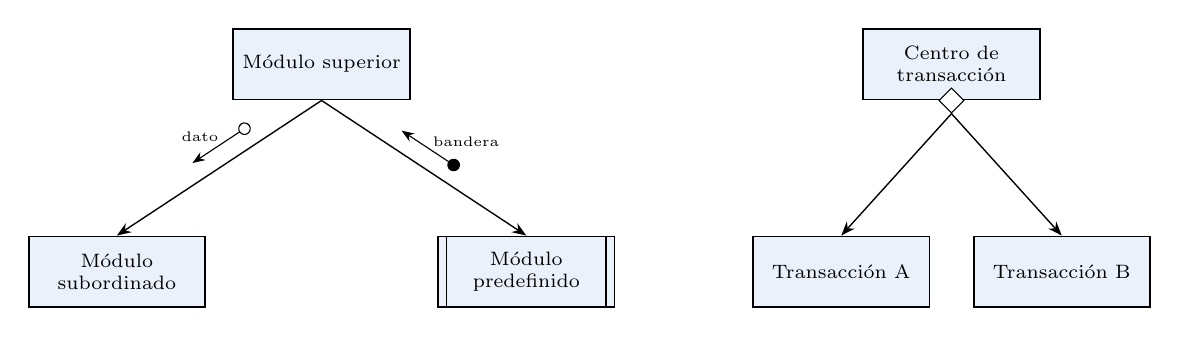
\begin{tikzpicture}[y = 1.2cm]
        \node[modulo] (A) at (0, 0) {Módulo superior};
        \node[modulo] (B) at (-2.6, -2.2) {Módulo\\subordinado};
        \node[predefinido] (C) at (2.6, -2.2) {Módulo\\predefinido};
        \conecta{A.south}{B.north} \baja{A.south}{B.north}{dato}
        \conecta{A.south}{C.north} \sube[control]{A.south}{C.north}{bandera}
        \node[modulo] (D) at (8.0, 0) {Centro de\\transacción};
        \node[seleccion] (SD) at (D.south) {};
        \node[modulo] (E) at (6.6, -2.2) {Transacción A};
        \node[modulo] (F) at (9.4, -2.2) {Transacción B};
        \draw[llamada] (SD.south) -- (E.north);
        \draw[llamada] (SD.south) -- (F.north);
    \end{tikzpicture}
    \caption[Notación del diagrama de estructura]{Notación del diagrama de estructura
    utilizada: llamada, acoplamiento de datos, bandera de control, módulo predefinido y
    selección.}
    \label{fig:de-notacion}
\end{figure}

% =========================================================
\section{Derivación desde los diagramas de flujo de datos}

La arquitectura se obtuvo aplicando las dos estrategias clásicas del diseño estructurado
sobre los DFD de la Parte~1:

\begin{itemize}
    \item \textbf{Análisis de transacción.} El DFD de nivel~0 muestra que BeeTracer no procesa
    un único flujo, sino seis tipos de solicitud independientes, una por cada proceso
    principal. Por ello el módulo principal se diseñó como un \emph{centro de transacción}
    (Figura~\ref{fig:de-general}): obtiene y autentica la solicitud, la despacha al subsistema
    que corresponde y muestra el resultado. Cada subsistema equivale a un proceso del nivel~0
    y conserva su nombre, lo que mantiene la trazabilidad entre análisis y diseño. Los
    subsistemas 1, 3, 4, 5 y 6 repiten el mismo patrón internamente, porque sus DFD de
    nivel~1 también reciben acontecimientos distintos que activan subprocesos distintos.
    \item \textbf{Análisis de transformación.} El subsistema Importar manifiesto
    (Figura~\ref{fig:de-importar}) sí tiene un flujo principal único que se transforma por
    etapas, por lo que se dividió en una rama \emph{aferente} (obtener el manifiesto
    válido: leer la solicitud, verificar duplicados, descargar el XML y validarlo), un
    \emph{centro de transformación} (registrar el manifiesto, que corresponde al DFD de
    nivel~2 del proceso 2.3) y una rama \emph{eferente} (emitir el resultado: reporte de
    errores, notificación a Aduanas y resumen).
\end{itemize}

Los procesos elementales de los DFD se convirtieron, en general, en módulos subordinados con
el mismo nombre (por ejemplo, \este{Contrastar cantidad} y \este{Evaluar diferencia} provienen
de los procesos 4.3.2 y 4.3.3). Además, aparecen módulos que no existían en el análisis
porque corresponden a la \textbf{tecnología de implementación} que el modelo esencial
excluyó: \este{Comprimir fotografía}, \este{Sellar fecha, hora y geoposición},
\este{Encolar fotografía} y \este{Sincronizar pendientes} resuelven el trabajo sin conexión en
el patio; \este{Descargar XML de Aduanas} y \este{Notificar a Aduanas} encapsulan el web
service del Servicio Nacional de Aduanas; \este{Enviar correo} encapsula el servidor de
correo; y \este{Generar PDF}, \este{Calcular hash de contraseña}, \este{Autenticar usuario} y
\este{Acceder a la base de datos} son servicios de biblioteca. Estos módulos corresponden a
las clases de servicio del Informe 2 (\clase{ServicioAduana}, \clase{ServicioCorreo} y
\clase{SincronizadorOffline}).

% =========================================================
\section{Criterios de calidad del diseño}

El diseño se evaluó con los criterios de acoplamiento y cohesión de
\textcite{yourdon1979}:

\begin{itemize}
    \item \textbf{Acoplamiento bajo.} Los módulos se comunican casi exclusivamente mediante
    acoplamientos de datos (identificadores, imágenes, listas) y no comparten datos
    globales. Las banderas de control se limitan a informar resultados hacia arriba
    (\este{válido}, \este{disponible}, \este{completa}, \este{autenticado}), nunca a indicar
    al subordinado qué hacer, lo que evita el acoplamiento de control descendente.
    \item \textbf{Cohesión funcional.} Cada módulo realiza una sola función que puede
    describirse con un verbo y un objeto. Por ejemplo, \este{Verificar disponibilidad} solo
    verifica y no registra; el registro lo hace \este{Registrar asignación}.
    \item \textbf{Fan-in en lugar de duplicación.} La lógica que se repite en varios casos se
    concentra en un solo módulo reutilizado: \este{Registrar evidencia fotográfica} es
    invocado por los cuatro módulos que capturan fotografías, lo que garantiza que la regla
    de evidencia obligatoria se aplique de la misma forma en todas las etapas;
    \este{Guardar registro maestro}, \este{Verificar conflicto de agenda} y
    \este{Filtrar operaciones} cumplen el mismo papel en sus subsistemas.
    \item \textbf{Fan-out acotado.} Los módulos invocan a siete subordinados o menos, con
    una excepción justificada: \este{Administrar datos maestros} tiene ocho, pero cinco de
    ellos son alternativas excluyentes de una misma selección y en cada transacción solo se
    ejecuta una. Cuando un subsistema crecía, se agregó un nivel intermedio (por ejemplo,
    \este{Obtener manifiesto válido} o \este{Registrar manifiesto}).
\end{itemize}

% =========================================================
\section{Diagramas}

A continuación se presentan el panorama general y el diagrama de cada uno de los seis
subsistemas. En las llamadas que se repiten con los mismos acoplamientos (por ejemplo, las
cinco llamadas a \este{Guardar registro maestro}), estos se dibujan una sola vez.

\diagramaapaisado{de_general}
    {Diagrama de estructura - Panorama general}
    {Diagrama de estructura - Panorama general (centro de transacción).}
    {fig:de-general}
\diagramaapaisado{de_maestros}
    {Diagrama de estructura - Administrar datos maestros}
    {Diagrama de estructura - Subsistema 1: Administrar datos maestros.}
    {fig:de-maestros}
\diagramaapaisado{de_importar}
    {Diagrama de estructura - Importar manifiesto}
    {Diagrama de estructura - Subsistema 2: Importar manifiesto (análisis de transformación).}
    {fig:de-importar}
\diagramaapaisado{de_programar}
    {Diagrama de estructura - Programar faenas}
    {Diagrama de estructura - Subsistema 3: Programar faenas.}
    {fig:de-programar}
\diagramaapaisado{de_operacion}
    {Diagrama de estructura - Ejecutar operación en terreno}
    {Diagrama de estructura - Subsistema 4: Ejecutar operación en terreno (aplicación móvil).}
    {fig:de-operacion}
\diagramaapaisado{de_validar}
    {Diagrama de estructura - Validar reporte}
    {Diagrama de estructura - Subsistema 5: Validar reporte.}
    {fig:de-validar}
\diagramaapaisado{de_distribuir}
    {Diagrama de estructura - Distribuir y consultar reportes}
    {Diagrama de estructura - Subsistema 6: Distribuir y consultar reportes.}
    {fig:de-distribuir}

\chapter{Modelo relacional}
\label{cap:relacional}

El modelo relacional traduce el diagrama entidad-relación (Sección~\ref{sec:der}) a un conjunto
de tablas listas para implementarse en un motor de base de datos relacional
\parencite{codd1970, elmasri2016}. Se aplicaron las reglas habituales de transformación:

\begin{enumerate}
    \item Cada \textbf{entidad} se convierte en una tabla, con sus atributos como columnas y su
    identificador como clave primaria (PK).
    \item Cada relación \textbf{1:N} se implementa agregando, en la tabla del lado N, una clave
    foránea (FK) que referencia a la clave primaria del lado 1 (por ejemplo,
    \texttt{LINEA\_CARGA.id\_contenedor}).
    \item Cada relación \textbf{1:1} se implementa con una clave foránea con restricción de
    unicidad en la tabla dependiente (por ejemplo, \texttt{OPERACION.id\_programacion} es FK y
    única, porque una programación origina una sola operación).
    \item La relación \textbf{N:M} entre \textsc{rol} y \textsc{permiso} se implementa con la
    tabla asociativa \texttt{ROL\_PERMISO}, cuya clave primaria compuesta está formada por las
    dos claves foráneas.
    \item Las \textbf{participaciones opcionales} del DER se implementan con claves foráneas que
    admiten nulo (por ejemplo, \texttt{PROGRAMACION.id\_cuadrilla} mientras la faena no está
    asignada, o \texttt{CONTENEDOR.id\_manifiesto} en tarja ciega).
\end{enumerate}

\section{Esquema relacional}

A continuación se presenta el esquema en notación textual: la clave primaria va
\uline{subrayada}, las claves foráneas en \textit{cursiva} con la tabla que referencian, y
\texttt{?} indica que la columna admite nulo. La columna \texttt{estado} de cada tabla toma su
dominio del diccionario de datos (\texttt{estado\_faena}, \texttt{estado\_sello},
\texttt{estado\_foto} o \texttt{estado\_reporte}, según corresponda).

{\small
\begin{itemize}
    \item \textbf{ROL}(\uline{id\_rol}, nombre, activo)
    \item \textbf{PERMISO}(\uline{id\_permiso}, codigo, descripcion)
    \item \textbf{ROL\_PERMISO}(\uline{\textit{id\_rol}}$\rightarrow$ROL,
    \uline{\textit{id\_permiso}}$\rightarrow$PERMISO)
    \item \textbf{CLIENTE}(\uline{id\_cliente}, rut, razon\_social, email, activo)
    \item \textbf{CUADRILLA}(\uline{id\_cuadrilla}, nombre)
    \item \textbf{TRABAJADOR}(\uline{id\_trabajador}, rut, nombre, cargo, habilitado,
    \textit{id\_cuadrilla}?$\rightarrow$CUADRILLA)
    \item \textbf{USUARIO}(\uline{id\_usuario}, nombre, email, password\_hash, activo,
    \textit{id\_rol}$\rightarrow$ROL, \textit{id\_trabajador}?$\rightarrow$TRABAJADOR,
    \textit{id\_cliente}?$\rightarrow$CLIENTE)
    \item \textbf{TIPO\_BULTO}(\uline{id\_tipo\_bulto}, codigo, nombre, activo)
    \item \textbf{MANIFIESTO}(\uline{id\_manifiesto}, numero, nave, viaje, fecha\_recepcion)
    \item \textbf{CONTENEDOR}(\uline{id\_contenedor}, numero, tamano, nro\_sello\_declarado,
    fecha\_arribo, \textit{id\_manifiesto}?$\rightarrow$MANIFIESTO)
    \item \textbf{LINEA\_CARGA}(\uline{id\_linea}, descripcion, cantidad\_declarada,
    cantidad\_recibida, \textit{id\_contenedor}$\rightarrow$CONTENEDOR,
    \textit{id\_cliente}$\rightarrow$CLIENTE, \textit{id\_tipo\_bulto}$\rightarrow$TIPO\_BULTO)
    \item \textbf{PROGRAMACION}(\uline{id\_programacion}, fecha, hora\_inicio, hora\_termino,
    estado, \textit{id\_contenedor}$\rightarrow$CONTENEDOR,
    \textit{id\_cuadrilla}?$\rightarrow$CUADRILLA,
    \textit{id\_jefe\_tarjador}?$\rightarrow$TRABAJADOR)
    \item \textbf{OPERACION}(\uline{id\_operacion}, hora\_inicio, hora\_fin?, estado,
    modalidad\_ingreso, \textit{id\_programacion}$\rightarrow$PROGRAMACION)
    \item \textbf{SELLO\_SEGURIDAD}(\uline{id\_sello}, numero\_digitado, estado,
    fecha\_verificacion, \textit{id\_operacion}$\rightarrow$OPERACION)
    \item \textbf{INCIDENCIA}(\uline{id\_incidencia}, tipo, descripcion, cantidad\_afectada,
    fecha\_hora, \textit{id\_operacion}$\rightarrow$OPERACION,
    \textit{id\_linea}?$\rightarrow$LINEA\_CARGA)
    \item \textbf{FOTOGRAFIA}(\uline{id\_foto}, uuid, etapa, fecha\_hora\_captura, latitud,
    longitud, url?, estado, motivo\_rechazo?, \textit{id\_operacion}$\rightarrow$OPERACION,
    \textit{id\_linea}?$\rightarrow$LINEA\_CARGA,
    \textit{id\_incidencia}?$\rightarrow$INCIDENCIA)
    \item \textbf{REPORTE}(\uline{id\_reporte}, folio, version, estado, fecha\_generacion,
    fecha\_aprobacion?, estado\_envio, documento\_pdf,
    \textit{id\_operacion}$\rightarrow$OPERACION, \textit{id\_aprobador}?$\rightarrow$USUARIO)
    \item \textbf{ENVIO\_REPORTE}(\uline{id\_envio}, fecha\_hora, destinatarios, origen,
    resultado, \textit{id\_reporte}$\rightarrow$REPORTE)
\end{itemize}
}

La Figura~\ref{fig:relacional} muestra las mismas tablas y sus claves foráneas; cada flecha
va desde la tabla que contiene la clave foránea hacia la tabla referenciada.

\diagramaapaisado{relacional}
    {Modelo relacional}
    {Modelo relacional del sistema BeeTracer.}
    {fig:relacional}

\section{Restricciones de integridad}

Además de las claves primarias y foráneas, el modelo incorpora las restricciones de la
Tabla~\ref{tab:restricciones}, que llevan a la base de datos las reglas de negocio
identificadas en las mini especificaciones.

{\estilotabla
\begin{longtable}{|L{3.4cm}|L{11.2cm}|}
\caption{Restricciones de integridad del modelo relacional.}
\label{tab:restricciones}\\
\hline
\rowcolor{filacabecera}
\textbf{Tabla} & \textbf{Restricción} \\ \hline
\endfirsthead
\hline
\rowcolor{filacabecera}
\textbf{Tabla} & \textbf{Restricción} \\ \hline
\endhead
USUARIO & \texttt{email} único. Si el rol es de jefe tarjador, \texttt{id\_trabajador} no
es nulo y es único; si es de cliente, \texttt{id\_cliente} no es nulo. \\ \hline
CLIENTE, TRABAJADOR & \texttt{rut} único y con formato válido (dominio \texttt{rut}). \\
\hline
PERMISO, TIPO\_BULTO & \texttt{codigo} único. \\ \hline
MANIFIESTO & Par (\texttt{nave}, \texttt{viaje}) único: un viaje se importa una sola vez. \\
\hline
CONTENEDOR & \texttt{numero} con formato ISO 6346; \texttt{tamano} $\in$ \{20, 40\}. \\
\hline
LINEA\_CARGA & \texttt{cantidad\_declarada} $\geq 1$; \texttt{cantidad\_recibida}
$\geq 0$. \\ \hline
PROGRAMACION & \texttt{id\_contenedor} único (un contenedor tiene una sola programación);
\texttt{hora\_inicio} $<$ \texttt{hora\_termino}; \texttt{estado} $\in$
\texttt{estado\_faena}. \\ \hline
OPERACION & \texttt{id\_programacion} único; \texttt{hora\_fin} no nulo cuando
\texttt{estado} = FINALIZADA. \\ \hline
SELLO\_SEGURIDAD & \texttt{id\_operacion} único (un sello por operación). \\ \hline
INCIDENCIA & \texttt{id\_linea} nulo solo si \texttt{tipo} = SELLO\_ALTERADO;
\texttt{cantidad\_afectada} $\geq 1$. \\ \hline
FOTOGRAFIA & \texttt{uuid} único; \texttt{id\_linea} no nulo si \texttt{etapa} = LOTE;
\texttt{id\_incidencia} no nulo si \texttt{etapa} = INCIDENCIA;
\texttt{motivo\_rechazo} no nulo si \texttt{estado} = RECHAZADA. \\ \hline
REPORTE & \texttt{folio} único; \texttt{id\_operacion} único; \texttt{version} $\geq 1$;
\texttt{id\_aprobador} y \texttt{fecha\_aprobacion} no nulos si \texttt{estado} =
APROBADO. \\ \hline
Borrado (todas) & Las claves foráneas usan \texttt{ON DELETE RESTRICT}: un registro
referenciado no puede eliminarse físicamente, y los datos maestros usados se desactivan
(eliminación lógica). La única excepción es \texttt{ROL\_PERMISO}, que usa \texttt{ON
DELETE CASCADE} al eliminar un rol sin usuarios. \\ \hline
\end{longtable}
}

\chapter{Especificaciones de cada módulo}
\label{cap:modulos}

Este capítulo especifica los módulos de los diagramas de estructura del
Capítulo~\ref{cap:estructura}. Mientras las mini especificaciones describen \emph{qué} hace
cada proceso del modelo esencial, las especificaciones de módulos describen \emph{cómo} se
organiza el programa: quién invoca a cada módulo, qué parámetros recibe y devuelve (sus
acoplamientos) y qué pasos ejecuta.

Para cada subsistema se presenta primero una tabla con todos sus módulos y luego la
especificación detallada, en pseudocódigo, de sus módulos de control y de los módulos que
concentran las reglas de negocio. Las banderas de control se escriben en
\texttt{monoespaciado}. Los módulos que implementan un proceso elemental siguen la lógica de
su mini especificación (Sección~\ref{sec:minispec}), que se indica entre paréntesis.

% =========================================================
\section{Módulo principal}

\tablamodulos{Módulos del panorama general.}{tab:mod-general}{%
Sistema BeeTracer & Ninguno (raíz) & Ninguna & Ninguna & Centro de transacción: obtiene la
solicitud, la despacha y muestra el resultado. \\ \hline
Obtener transacción & Sistema BeeTracer & Ninguna & solicitud & Lee la solicitud y
autentica al usuario. \\ \hline
Leer solicitud & Obtener transacción & Ninguna & solicitud & Captura la solicitud desde la
interfaz web o móvil. \\ \hline
Despachar transacción & Sistema BeeTracer & solicitud & resultado & Selecciona el
subsistema según el tipo de transacción. \\ \hline
Mostrar resultado & Sistema BeeTracer & resultado & Ninguna & Presenta la respuesta en la
interfaz que originó la solicitud. \\ \hline
}

\begin{modspec}{Sistema BeeTracer}
\msdato{Llama a}{Obtener transacción, Despachar transacción, Mostrar resultado.}
\msdato{Entradas / salidas}{Ninguna (módulo raíz).}
\textbf{Proceso:}
\begin{logica}
    \item \kw{REPETIR} mientras el sistema esté en servicio:
    \begin{logica}
        \item Obtener transacción $\rightarrow$ solicitud, \texttt{autenticado}.
        \item \kw{SI} \texttt{autenticado} = falso \kw{ENTONCES} resultado = ``acceso
        denegado'' \kw{SINO SI} el rol del usuario no tiene el permiso de la transacción
        \kw{ENTONCES} resultado = ``operación no permitida'' \kw{SINO} Despachar
        transacción(solicitud) $\rightarrow$ resultado.
        \item Mostrar resultado(resultado).
    \end{logica}
\end{logica}
\end{modspec}

\begin{modspec}{Despachar transacción}
\msdato{Llamado por}{Sistema BeeTracer.}
\msdato{Llama a}{Los seis subsistemas (selección).}
\msdato{Entradas}{solicitud. \textbf{Salidas:} resultado.}
\textbf{Proceso:}
\begin{logica}
    \item \kw{SEGÚN} el tipo de solicitud:
    \begin{logica}
        \item mantención de datos maestros $\rightarrow$ Administrar datos maestros.
        \item importación $\rightarrow$ Importar manifiesto.
        \item programación o consulta de faenas asignadas $\rightarrow$ Programar faenas.
        \item registro de terreno $\rightarrow$ Ejecutar operación en terreno.
        \item revisión, decisión o reemplazo de evidencia $\rightarrow$ Validar reporte.
        \item reenvío o consulta de operaciones y reportes $\rightarrow$ Distribuir y
        consultar reportes.
    \end{logica}
    \item \kw{SI} Ejecutar operación en terreno devuelve \texttt{finalizada} \kw{ENTONCES}
    invocar Validar reporte con la transacción ``generar borrador''.
    \item \kw{SI} Validar reporte devuelve \texttt{aprobado} \kw{ENTONCES} invocar
    Distribuir y consultar reportes con la transacción ``enviar reporte''.
    \item Retornar resultado.
\end{logica}
\end{modspec}

% =========================================================
\section{Subsistema 1: Administrar datos maestros}

\tablamodulos{Módulos del subsistema Administrar datos maestros.}{tab:mod-maestros}{%
Administrar datos maestros & Despachar transacción & solicitud de mantención & resultado de
mantención & Valida y selecciona la mantención según el tipo de dato maestro. \\ \hline
Leer solicitud de mantención & Administrar datos maestros & Ninguna & solicitud & Lee el
formulario y la acción solicitada. \\ \hline
Validar datos maestros & Administrar datos maestros & solicitud & \texttt{válido}, errores
& Verifica campos obligatorios y formatos. \\ \hline
Mantener usuario & Administrar datos maestros & datos de usuario & resultado & Aplica la
acción sobre el usuario (mini especificación 1.1). \\ \hline
Mantener rol y permisos & Administrar datos maestros & datos de rol & resultado & Aplica la
acción sobre el rol y sus permisos (1.2). \\ \hline
Mantener tipo de bulto & Administrar datos maestros & datos de tipo de bulto & resultado &
Aplica la acción sobre el tipo de bulto (1.3). \\ \hline
Mantener cliente & Administrar datos maestros & datos de cliente & resultado & Aplica la
acción sobre el cliente (1.4). \\ \hline
Mantener trabajador y cuadrilla & Administrar datos maestros & datos de trabajador &
resultado & Aplica la acción sobre el trabajador o la cuadrilla (1.5). \\ \hline
Mostrar resultado de mantención & Administrar datos maestros & resultado & Ninguna &
Informa el éxito o los errores al Administrador. \\ \hline
}

\begin{modspec}{Administrar datos maestros}
\msdato{Llamado por}{Despachar transacción.}
\msdato{Llama a}{Leer solicitud de mantención, Validar datos maestros, los cinco módulos
Mantener (selección), Mostrar resultado de mantención.}
\msdato{Entradas}{solicitud de mantención. \textbf{Salidas:} resultado de mantención.}
\textbf{Proceso:}
\begin{logica}
    \item Leer solicitud de mantención $\rightarrow$ solicitud.
    \item Validar datos maestros(solicitud) $\rightarrow$ \texttt{válido}, errores.
    \item \kw{SI} \texttt{válido} = falso \kw{ENTONCES} resultado = errores \kw{SINO SEGÚN}
    el tipo de dato maestro invocar Mantener usuario, Mantener rol y permisos, Mantener tipo
    de bulto, Mantener cliente o Mantener trabajador y cuadrilla $\rightarrow$ resultado.
    \item Mostrar resultado de mantención(resultado).
\end{logica}
\end{modspec}

\begin{modspec}{Validar datos maestros}
\msdato{Llamado por}{Administrar datos maestros.}
\msdato{Llama a}{Validar RUT, Validar email.}
\msdato{Entradas}{solicitud. \textbf{Salidas:} \texttt{válido}, errores.}
\textbf{Proceso:}
\begin{logica}
    \item errores = lista vacía.
    \item \kw{PARA CADA} campo obligatorio de la acción: \kw{SI} está vacío \kw{ENTONCES}
    agregar ``campo obligatorio'' a errores.
    \item \kw{SI} la solicitud incluye rut \kw{ENTONCES} Validar RUT(rut) $\rightarrow$
    \texttt{rut válido}; \kw{SI} es falso, agregar el error.
    \item \kw{SI} la solicitud incluye email \kw{ENTONCES} Validar email(email)
    $\rightarrow$ \texttt{email válido}; \kw{SI} es falso, agregar el error.
    \item \texttt{válido} = (errores está vacía); retornar \texttt{válido} y errores.
\end{logica}
\end{modspec}

% =========================================================
\section{Subsistema 2: Importar manifiesto}

\tablamodulos{Módulos del subsistema Importar manifiesto.}{tab:mod-importar}{%
Importar manifiesto & Despachar transacción & solicitud de importación & resultado de
importación & Coordina las ramas aferente, central y eferente. \\ \hline
Obtener manifiesto válido & Importar manifiesto & Ninguna & manifiesto válido,
\texttt{válido}, errores & Rama aferente: obtiene y valida el XML. \\ \hline
Leer solicitud de importación & Obtener manifiesto válido & Ninguna & nave, viaje, fecha &
Lee los datos del viaje (2.1). \\ \hline
Verificar importación previa & Obtener manifiesto válido & nave, viaje &
\texttt{duplicado} & Busca un manifiesto del mismo viaje (2.1). \\ \hline
Validar estructura y datos & Obtener manifiesto válido & xml & \texttt{válido}, errores &
Valida esquema, contenedores y líneas (2.2). \\ \hline
Registrar manifiesto & Importar manifiesto & manifiesto válido & resumen & Centro de
transformación: registra cabecera, contenedores y líneas (2.3). \\ \hline
Registrar cabecera & Registrar manifiesto & cabecera & id\_manifiesto & Escribe el
manifiesto (2.3.1). \\ \hline
Registrar contenedores & Registrar manifiesto & contenedores, id\_manifiesto &
\{id\_contenedor\} & Escribe los contenedores (2.3.2). \\ \hline
Verificar consignatario & Registrar manifiesto & rut, razon\_social & id\_cliente, advertencia
& Busca o crea el cliente (2.3.3). \\ \hline
Registrar líneas de carga & Registrar manifiesto & líneas & cantidad\_lineas & Escribe las
líneas (2.3.4). \\ \hline
Emitir resultado de importación & Importar manifiesto & resumen o errores & Ninguna & Rama
eferente: informa a Aduanas y al Jefe de faena. \\ \hline
Generar reporte de errores & Emitir resultado de importación & errores & reporte de errores
& Compone el reporte (2.4). \\ \hline
Mostrar resumen de importación & Emitir resultado de importación & resumen & Ninguna &
Presenta el resumen al Jefe de faena (2.5). \\ \hline
}

\begin{modspec}{Importar manifiesto}
\msdato{Llamado por}{Despachar transacción.}
\msdato{Llama a}{Obtener manifiesto válido, Registrar manifiesto, Emitir resultado de
importación.}
\msdato{Entradas}{solicitud de importación. \textbf{Salidas:} resultado de importación.}
\textbf{Proceso:}
\begin{logica}
    \item Obtener manifiesto válido $\rightarrow$ manifiesto válido, \texttt{válido}, errores.
    \item \kw{SI} \texttt{válido} \kw{ENTONCES} Registrar manifiesto(manifiesto válido)
    $\rightarrow$ resumen; Emitir resultado de importación(resumen).
    \item \kw{SINO} Emitir resultado de importación(errores).
\end{logica}
\end{modspec}

\begin{modspec}{Obtener manifiesto válido}
\msdato{Llamado por}{Importar manifiesto.}
\msdato{Llama a}{Leer solicitud de importación, Verificar importación previa, Descargar XML
de Aduanas, Validar estructura y datos.}
\msdato{Entradas}{Ninguna. \textbf{Salidas:} manifiesto válido, \texttt{válido}, errores.}
\textbf{Proceso:}
\begin{logica}
    \item Leer solicitud de importación $\rightarrow$ nave, viaje, fecha, reemplazar.
    \item Verificar importación previa(nave, viaje) $\rightarrow$ \texttt{duplicado}.
    \item \kw{SI} \texttt{duplicado} y no reemplazar \kw{ENTONCES} retornar \texttt{válido} =
    falso con el aviso de importación duplicada.
    \item Descargar XML de Aduanas(nave, viaje, fecha) $\rightarrow$ xml; \kw{SI} el servicio
    no responde, retornar \texttt{válido} = falso con ``manifiesto no disponible''.
    \item Validar estructura y datos(xml) $\rightarrow$ \texttt{válido}, errores; retornar.
\end{logica}
\end{modspec}

% =========================================================
\section{Subsistema 3: Programar faenas}

\tablamodulos{Módulos del subsistema Programar faenas.}{tab:mod-programar}{%
Programar faenas & Despachar transacción & datos de programación o credenciales &
confirmación o faenas asignadas & Selecciona la transacción de programación. \\ \hline
Leer solicitud de programación & Programar faenas & Ninguna & solicitud & Lee el formulario
o la consulta de la aplicación móvil. \\ \hline
Crear programación & Programar faenas & datos de nueva programación & id\_programacion &
Crea la programación (3.1). \\ \hline
Modificar programación & Programar faenas & cambio de programación & confirmación &
Reprograma, anula, elimina o cambia el estado (3.3). \\ \hline
Verificar conflicto de agenda & Crear y Modificar programación & franja, id\_contenedor &
\texttt{conflicto} & Detecta cruces con otras programaciones. \\ \hline
Asignar cuadrilla y jefe tarjador & Programar faenas & datos de asignación & confirmación &
Coordina la asignación (3.2). \\ \hline
Determinar recursos disponibles & Asignar cuadrilla y jefe tarjador & id\_programacion &
recursos disponibles & Lista cuadrillas y jefes libres (3.2.1). \\ \hline
Verificar disponibilidad & Asignar cuadrilla y jefe tarjador & selección &
\texttt{disponible} & Revalida la selección (3.2.2). \\ \hline
Registrar asignación & Asignar cuadrilla y jefe tarjador & asignación & Ninguna & Guarda la
asignación (3.2.3). \\ \hline
Entregar faenas asignadas & Programar faenas & credenciales & faenas asignadas & Entrega
las faenas al jefe tarjador (3.4). \\ \hline
Obtener faenas del jefe tarjador & Entregar faenas asignadas & id\_trabajador & faenas &
Lee programaciones y carga declarada. \\ \hline
Mostrar confirmación & Programar faenas & confirmación & Ninguna & Presenta el resultado. \\
\hline
}

\begin{modspec}{Asignar cuadrilla y jefe tarjador}
\msdato{Llamado por}{Programar faenas.}
\msdato{Llama a}{Determinar recursos disponibles, Verificar disponibilidad, Registrar
asignación.}
\msdato{Entradas}{datos de asignación. \textbf{Salidas:} confirmación de programación.}
\textbf{Proceso:}
\begin{logica}
    \item \kw{SI} los datos son una solicitud de recursos \kw{ENTONCES} Determinar recursos
    disponibles(id\_programacion) $\rightarrow$ recursos; retornar recursos.
    \item \kw{SINO} Verificar disponibilidad(selección) $\rightarrow$ \texttt{disponible}.
    \item \kw{SI} \texttt{disponible} \kw{ENTONCES} Registrar asignación(selección) y
    retornar ``asignación registrada'' \kw{SINO} retornar ``rechazo de asignación''
    indicando el recurso no disponible.
\end{logica}
\end{modspec}

\begin{modspec}{Verificar conflicto de agenda}
\msdato{Llamado por}{Crear programación, Modificar programación (fan-in).}
\msdato{Llama a}{Acceder a la base de datos.}
\msdato{Entradas}{fecha, hora\_inicio, hora\_termino, id\_contenedor. \textbf{Salidas:}
\texttt{conflicto}.}
\textbf{Proceso:}
\begin{logica}
    \item Leer las programaciones del mismo contenedor o de la misma fecha que no estén
    ANULADAS ni FINALIZADAS, excluyendo la que se está modificando.
    \item \texttt{conflicto} = existe alguna con el mismo contenedor, o alguna cuyo intervalo
    [hora\_inicio, hora\_termino) se intersecta con el nuevo y comparte cuadrilla o jefe
    tarjador.
    \item Retornar \texttt{conflicto}.
\end{logica}
\end{modspec}

% =========================================================
\section{Subsistema 4: Ejecutar operación en terreno}

Este subsistema se ejecuta en la aplicación móvil. A diferencia del modelo esencial, el
diseño incorpora el trabajo sin conexión: cada fotografía se comprime, se sella y se encola
localmente, y se envía de inmediato si hay señal o al recuperarla.

\tablamodulos{Módulos del subsistema Ejecutar operación en terreno.}{tab:mod-operacion}{%
Ejecutar operación en terreno & Despachar transacción & registro de terreno & confirmación
de registro, \texttt{finalizada} & Selecciona la etapa del flujo guiado. \\ \hline
Leer registro de terreno & Ejecutar operación en terreno & Ninguna & registro & Lee los
datos e imágenes de la etapa actual. \\ \hline
Iniciar operación & Ejecutar operación en terreno & datos de inicio & confirmación & Crea la
operación (4.1). \\ \hline
Verificar sello & Ejecutar operación en terreno & datos de sello & estado\_sello &
Compara el sello y exige incidencia si no está intacto (4.2). \\ \hline
Registrar lote & Ejecutar operación en terreno & datos de lote & confirmación & Identifica
la línea y coordina el contraste (4.3). \\ \hline
Contrastar cantidad & Registrar lote & id\_linea, cantidad & diferencia & Acumula lo
recibido (4.3.2). \\ \hline
Evaluar diferencia & Registrar lote & diferencia, dano\_visible &
\texttt{incidencia requerida} & Decide si se exige incidencia (4.3.3). \\ \hline
Registrar incidencia & Ejecutar operación en terreno & datos de incidencia & id\_incidencia &
Registra el hallazgo (4.4). \\ \hline
Registrar evidencia fotográfica & Verificar sello, Registrar lote, Registrar incidencia,
Cerrar faena & imagen, etapa, referencias & id\_foto & Aplica la regla de evidencia
obligatoria. \\ \hline
Cerrar faena & Ejecutar operación en terreno & datos de cierre & \texttt{finalizada} &
Verifica evidencia, registra faltantes y cierra (4.5). \\ \hline
Verificar evidencia obligatoria & Cerrar faena & id\_operacion & \texttt{completa}, etapas
faltantes & Revisa que existan las etapas obligatorias. \\ \hline
Registrar faltantes & Cerrar faena & líneas incompletas & Ninguna & Crea incidencias
FALTANTE confirmadas. \\ \hline
Mostrar confirmación & Ejecutar operación en terreno & confirmación & Ninguna & Indica la
siguiente etapa del flujo guiado. \\ \hline
}

\begin{modspec}{Registrar evidencia fotográfica}
\msdato{Llamado por}{Verificar sello, Registrar lote, Registrar incidencia, Cerrar faena
(fan-in).}
\msdato{Llama a}{Comprimir fotografía, Sellar fecha, hora y geoposición, Encolar fotografía.}
\msdato{Entradas}{imagen, etapa, id\_operacion, (id\_linea), (id\_incidencia).
\textbf{Salidas:} id\_foto.}
\textbf{Proceso:}
\begin{logica}
    \item \kw{SI} la imagen está vacía o es ilegible \kw{ENTONCES} retornar error: no se
    permite avanzar sin una fotografía válida.
    \item Comprimir fotografía(imagen) $\rightarrow$ imagen comprimida.
    \item Sellar fecha, hora y geoposición(imagen comprimida) $\rightarrow$ fotografía con
    uuid, fecha\_hora\_captura, latitud y longitud.
    \item Guardar la fotografía en la base local con estado = PENDIENTE y sus referencias.
    \item Encolar fotografía(fotografía): si hay conectividad se sube de inmediato y pasa a
    SUBIDA; si no, permanece en la cola.
    \item Retornar id\_foto.
\end{logica}
\end{modspec}

\begin{modspec}{Cerrar faena}
\msdato{Llamado por}{Ejecutar operación en terreno.}
\msdato{Llama a}{Registrar evidencia fotográfica, Verificar evidencia obligatoria,
Registrar faltantes, Sincronizar pendientes.}
\msdato{Entradas}{datos de cierre. \textbf{Salidas:} confirmación de registro,
\texttt{finalizada}.}
\textbf{Proceso:}
\begin{logica}
    \item Registrar evidencia fotográfica(imagen, etapa = CIERRE).
    \item Verificar evidencia obligatoria(id\_operacion) $\rightarrow$ \texttt{completa};
    \kw{SI} es falsa, retornar las etapas faltantes con \texttt{finalizada} = falso.
    \item \kw{SI} hay líneas con cantidad\_recibida $<$ cantidad\_declarada \kw{ENTONCES}
    pedir confirmación; \kw{SI} se confirma, Registrar faltantes(líneas) \kw{SINO} retornar
    sin cerrar.
    \item Sincronizar pendientes $\rightarrow$ cantidad enviada; las fotografías que no
    puedan enviarse se sincronizarán en segundo plano.
    \item Registrar hora\_fin y estado = FINALIZADA en la operación y en la programación.
    \item Retornar \texttt{finalizada} = verdadero.
\end{logica}
\end{modspec}

% =========================================================
\section{Subsistema 5: Validar reporte}

\tablamodulos{Módulos del subsistema Validar reporte.}{tab:mod-validar}{%
Validar reporte & Despachar transacción & solicitud de validación & reporte para revisión,
\texttt{aprobado} & Selecciona generar, presentar, aprobar, rechazar o reemplazar. \\ \hline
Leer solicitud de validación & Validar reporte & Ninguna & solicitud & Lee la acción del
Supervisor o del jefe tarjador. \\ \hline
Generar borrador de reporte & Validar reporte & id\_operacion & id\_reporte & Compone y
guarda el reporte (5.1). \\ \hline
Obtener datos de la operación & Generar borrador de reporte & id\_operacion & datos &
Lee operación, sello, incidencias y líneas. \\ \hline
Ordenar evidencia por etapa y cliente & Generar borrador de reporte & fotografías &
fotografías ordenadas & Agrupa por etapa y, en lotes, por cliente. \\ \hline
Presentar reporte & Validar reporte & id\_reporte & reporte & Muestra la bandeja o un
reporte (5.2). \\ \hline
Aprobar reporte & Validar reporte & id\_reporte, id\_aprobador & \texttt{aprobado} &
Aprueba si la evidencia está completa (5.3). \\ \hline
Verificar evidencia obligatoria & Aprobar reporte & id\_operacion & \texttt{completa} &
Revisa etapas y rechazos pendientes. \\ \hline
Registrar aprobación & Aprobar reporte & id\_reporte, id\_aprobador & Ninguna & Cambia el
estado a APROBADO. \\ \hline
Rechazar evidencia & Validar reporte & id\_foto, motivo & Ninguna & Rechaza y solicita
recaptura (5.4). \\ \hline
Marcar fotografía rechazada & Rechazar evidencia & id\_foto, motivo & Ninguna & Guarda
RECHAZADA y el motivo. \\ \hline
Reemplazar evidencia & Validar reporte & id\_foto, imagen & \texttt{corregida} & Registra
el reemplazo (5.5). \\ \hline
Registrar fotografía de reemplazo & Reemplazar evidencia & id\_foto, imagen & Ninguna &
Crea la nueva fotografía y marca la anterior REEMPLAZADA. \\ \hline
}

\begin{modspec}{Validar reporte}
\msdato{Llamado por}{Despachar transacción.}
\msdato{Llama a}{Leer solicitud de validación y, por selección, Generar borrador de reporte,
Presentar reporte, Aprobar reporte, Rechazar evidencia o Reemplazar evidencia.}
\msdato{Entradas}{solicitud de validación. \textbf{Salidas:} reporte para revisión,
\texttt{aprobado}.}
\textbf{Proceso:}
\begin{logica}
    \item Leer solicitud de validación $\rightarrow$ solicitud.
    \item \kw{SEGÚN} la acción: generar $\rightarrow$ Generar borrador de reporte; revisar
    $\rightarrow$ Presentar reporte; aprobar $\rightarrow$ Aprobar reporte; rechazar
    $\rightarrow$ Rechazar evidencia; reemplazar $\rightarrow$ Reemplazar evidencia.
    \item \kw{SI} Reemplazar evidencia retorna \texttt{corregida} \kw{ENTONCES} Generar
    borrador de reporte(id\_operacion) para crear la nueva versión.
    \item Retornar el resultado y, si corresponde, \texttt{aprobado} = verdadero.
\end{logica}
\end{modspec}

% =========================================================
\section{Subsistema 6: Distribuir y consultar reportes}

\tablamodulos{Módulos del subsistema Distribuir y consultar reportes.}{tab:mod-distribuir}{%
Distribuir y consultar reportes & Despachar transacción & solicitud & resultado &
Selecciona enviar, consultar o entregar. \\ \hline
Leer solicitud & Distribuir y consultar reportes & Ninguna & solicitud & Lee la solicitud
o los filtros. \\ \hline
Enviar reporte & Distribuir y consultar reportes & id\_reporte & resultado de envío &
Envía por correo y registra el envío (6.1). \\ \hline
Obtener destinatarios & Enviar reporte & id\_reporte & destinatarios & Correos de los
clientes con carga en la operación. \\ \hline
Registrar envío & Enviar reporte & resultado, destinatarios & Ninguna & Escribe el envío y
el estado\_envio. \\ \hline
Consultar operaciones & Distribuir y consultar reportes & consulta de operaciones & listado
de operaciones & Filtra y, si se pide, cambia el estado (6.2). \\ \hline
Modificar estado de operación & Consultar operaciones & id\_operacion, nuevo estado &
Ninguna & Cambia el estado si es una transición válida. \\ \hline
Filtrar operaciones & Consultar operaciones, Consultar estado del cliente & filtros &
operaciones & Aplica los filtros y, para clientes, restringe a su carga. \\ \hline
Consultar estado del cliente & Distribuir y consultar reportes & consulta de estado & estado
de operaciones & Atiende la consulta del cliente (6.3). \\ \hline
Entregar reporte PDF & Distribuir y consultar reportes & solicitud de PDF & reporte PDF &
Entrega el PDF aprobado (6.4). \\ \hline
Verificar acceso al reporte & Entregar reporte PDF & id\_reporte, id\_cliente &
\texttt{permitido} & Comprueba estado APROBADO y pertenencia. \\ \hline
Leer documento PDF & Entregar reporte PDF & id\_reporte & pdf & Recupera el documento
almacenado. \\ \hline
Mostrar resultado & Distribuir y consultar reportes & resultado & Ninguna & Presenta el
listado, el estado o el resultado del envío. \\ \hline
}

\begin{modspec}{Enviar reporte}
\msdato{Llamado por}{Distribuir y consultar reportes (envío automático o reenvío).}
\msdato{Llama a}{Obtener destinatarios, Enviar correo, Registrar envío.}
\msdato{Entradas}{id\_reporte, origen. \textbf{Salidas:} resultado de envío.}
\textbf{Proceso:}
\begin{logica}
    \item \kw{SI} el reporte no está APROBADO \kw{ENTONCES} retornar ``reporte pendiente de
    validación''.
    \item Obtener destinatarios(id\_reporte) $\rightarrow$ destinatarios.
    \item \kw{SI} destinatarios está vacía \kw{ENTONCES} resultado = FALLIDO, ``completar
    ficha del cliente''.
    \item \kw{SINO} Enviar correo(destinatarios, asunto, pdf) $\rightarrow$
    \texttt{aceptado}; resultado = ENVIADO \kw{SI} \texttt{aceptado} \kw{SINO} FALLIDO.
    \item Registrar envío(resultado, destinatarios, origen); retornar resultado.
\end{logica}
\end{modspec}

% =========================================================
\section{Módulos predefinidos}

Los módulos predefinidos son servicios de biblioteca o interfaces con sistemas externos que
el diseño reutiliza (Tabla~\ref{tab:mod-predefinidos}). Corresponden a las clases de servicio
del Informe 2 y concentran la tecnología que el modelo esencial había abstraído.

{\estilotabla
\begin{longtable}{|L{3.0cm}|L{3.2cm}|L{3.8cm}|L{4.6cm}|}
\caption{Módulos predefinidos del diseño.}
\label{tab:mod-predefinidos}\\
\hline
\rowcolor{filacabecera}
\textbf{Módulo} & \textbf{Entradas / salidas} & \textbf{Función} & \textbf{Implementación
(Informe 2)} \\ \hline
\endfirsthead
\hline
\rowcolor{filacabecera}
\textbf{Módulo} & \textbf{Entradas / salidas} & \textbf{Función} & \textbf{Implementación
(Informe 2)} \\ \hline
\endhead
Autenticar usuario & credenciales / \texttt{autenticado}, id\_usuario & Verifica email,
password\_hash y cuenta activa. & \clase{Usuario}:\newline \textit{iniciarSesion()} \\ \hline
Acceder a la base de datos & consulta / registros & Lee y escribe en las tablas del modelo
relacional. & Capa de persistencia \\ \hline
Validar RUT, Validar email & valor / \texttt{válido} & Verifican formato y dígito
verificador. & Biblioteca de validación \\ \hline
Calcular hash de contraseña & password / password\_hash & Genera el resumen criptográfico.
& \clase{Usuario}:\newline \textit{cambiarPassword()} \\ \hline
Guardar registro maestro & registro / \texttt{guardado} & Escribe o actualiza un dato
maestro. & Capa de persistencia \\ \hline
Descargar XML de Aduanas & nave, viaje, fecha / xml & Consume el web service del Servicio
Nacional de Aduanas. & \clase{ServicioAduana}:\newline \textit{descargarXML()} \\ \hline
Notificar a Aduanas & nave, viaje, resultado / -- & Informa el resultado de la
importación. & \clase{ServicioAduana}:\newline \textit{notificarResultadoImportacion()} \\ \hline
Comprimir fotografía & imagen / imagen comprimida & Reduce el tamaño antes del envío. &
\clase{Fotografia}:\newline \textit{comprimir()} \\ \hline
Sellar fecha, hora y geoposición & imagen / fotografía & Agrega uuid, fecha, hora,
latitud y longitud. & Servicios del dispositivo móvil \\ \hline
Encolar fotografía & fotografía / -- & Agrega a la cola local y envía si hay señal. &
\clase{SincronizadorOffline}:\newline \textit{encolar()} \\ \hline
Sincronizar pendientes & -- / cantidad enviada & Envía las fotografías encoladas. &
\clase{SincronizadorOffline}:\newline \textit{sincronizarPendientes()} \\ \hline
Generar PDF & contenido / pdf & Compila datos y fotografías en el documento. &
\clase{Reporte}:\newline \textit{generarPDF()} \\ \hline
Notificar a terreno & solicitud de recaptura / -- & Envía la solicitud a la aplicación
del jefe tarjador. & \clase{GestorReportes}:\newline \textit{solicitarCorreccionEvidencia()} \\ \hline
Enviar correo & destinatarios, asunto, pdf / \texttt{aceptado} & Entrega el correo al
servidor de salida. & \clase{ServicioCorreo}:\newline \textit{enviar()} \\ \hline
\end{longtable}
}

\chapter{Conclusiones}
\label{cap:conclusiones}

El objetivo de este informe fue modelar BeeTracer con el paradigma estructurado, dando
continuidad a la reconstrucción por ingeniería inversa iniciada en el Informe 2. El análisis
partió del entorno del sistema: la declaración de propósitos fijó su razón de ser, registrar de
forma verificable el estado de la carga en cada etapa del desconsolidado, y el diagrama de
contexto y la lista de acontecimientos delimitaron los seis terminadores y los veinticuatro
estímulos a los que debe responder. Desde allí, los diagramas de flujo de datos descompusieron
el sistema en seis procesos principales, veintiocho procesos de nivel~1 y diez de nivel~2, cuyos
flujos y almacenes quedaron definidos sin ambigüedad en el diccionario de datos y cuya lógica
quedó descrita en las mini especificaciones.

Comparar ambos enfoques sobre el mismo sistema fue la principal lección del trabajo. El modelo
orientado a objetos del Informe 2 organizaba el sistema en torno a \emph{quién} es responsable
de cada dato y comportamiento; el modelo estructurado lo organiza en torno a \emph{qué} se hace
con los datos y dónde quedan. Este cambio de perspectiva hizo visibles detalles que el
diagrama de clases no mostraba con claridad: la necesidad de registrar la etapa de cada
fotografía para ordenar el reporte, la conveniencia de registrar cada envío del reporte como
un hecho propio y la obligación de registrar el contenedor cuando se opera en tarja ciega. A
la vez, la trazabilidad entre ambos modelos se mantuvo: las entidades del DER coinciden con las
clases de entidad, y los módulos predefinidos del diseño, con las clases de servicio.

La distinción entre el modelo esencial y el diseño resultó especialmente útil en BeeTracer.
Al suponer tecnología perfecta, el análisis se concentró en las reglas de negocio (evidencia
obligatoria, contraste de cantidades, validación del supervisor) sin distraerse con la falta
de señal en el patio. En el diseño, esos aspectos tecnológicos se incorporaron como módulos
bien delimitados (compresión, sellado, encolado y sincronización de fotografías), y el
análisis de transacción permitió obtener una arquitectura en la que cada subsistema
corresponde a un proceso del nivel~0. El módulo \este{Registrar evidencia fotográfica},
reutilizado por todas las etapas, muestra cómo un buen diseño concentra en un solo lugar la
regla que da valor al producto.

Como limitación, al igual que en el informe anterior, no se tuvo acceso al código ni a la
base de datos de BeeTracer, por lo que los procesos, módulos y tablas propuestos son una
reconstrucción coherente con lo observado y no necesariamente idéntica a la implementación
real. Aun así, el modelo relacional y las especificaciones de módulos constituyen una base
concreta para una eventual implementación o para evaluar mejoras del sistema, como la
auditoría de los cambios de estado o la integración con los módulos complementarios que la
empresa comercializa por separado.


% =========================================================
% REFERENCIAS BIBLIOGRÁFICAS
% =========================================================

\clearpage
\chapter{Referencias bibliográficas}
\label{cap:referencias}

\nocite{*}
\printbibliography[heading=none]

\end{document}
